\documentclass[11pt, a4paper]{article}

\usepackage[utf8]{inputenc}
\usepackage{graphicx}
\graphicspath{ {images/} }
\usepackage{mathtools}
\usepackage{amssymb}
\usepackage{amsmath}
\usepackage[ngerman,english]{babel}
\usepackage{cite}
\usepackage{bibgerm}
\usepackage{fullpage}
\usepackage[top=1.5cm,bottom=1.5cm,left=3.5cm,right=2.5cm,headsep=1.5cm,includeheadfoot]{geometry}
\usepackage{tabularx}
\usepackage{caption}
\usepackage{subcaption}
\usepackage{eurosym}
\usepackage{enumitem}
\usepackage{multicol}
\usepackage{tikz}
\usepackage{tkz-euclide}
\usepackage{pgfplots}
\usepackage{pdflscape}
\usepackage{acronym}
\usepackage{blindtext}
\usepackage{ifthen}
\usepackage{setspace}
\usepackage{cancel}
\usepackage{color}
\usepackage{listings}
\usepackage{comment}
\usepackage{xcolor}
\usepackage{colortbl}
\usepackage[parfill]{parskip}
\usepackage{url}

\usepackage{fancyhdr}
\pagestyle{fancy}

\fancyhf{} % clear all
\fancyhead[L]{\leftmark}
\fancyfoot[C]{-- \thepage{} --}
\setlength{\headheight}{0pt}
\renewcommand{\headrulewidth}{0.5pt}
\renewcommand{\footrulewidth}{0pt}
\setlength{\skip\footins}{0.7cm}

\usetikzlibrary{shapes.geometric}
\usetikzlibrary{graphs}
\usetikzlibrary{positioning}

\onehalfspacing
\setlength\parindent{0pt}

%\everymath{\displaystyle}

\allowdisplaybreaks

\definecolor{AI-BLUE}{rgb}{0,0.57,0.87}
\definecolor{lightgray}{rgb}{0.91,0.91,0.91}

% Eigene Befehle
\newcommand\q[1]{\emph{"#1"}}
\renewcommand\equiv{\Leftrightarrow}
\newcommand\vertequal[2]{\underset{\underset{#2}{\parallel}}{#1}}
\newcommand\cif{\text{if }}
\newcommand\abs[1]{\left|#1\right|}
\newcommand\norm[1]{\abs{\abs{#1}}}
\newcommand\diff[1]{\text{ d#1}}
\newcommand\av[1]{\left\langle#1\right\rangle}
\newcommand\ev[1]{\mathbb{E}\left(#1\right)}
\newcommand\br[1]{\left(#1\right)}
\newcommand\ubr[2]{\underbrace{#1}_{#2}}
\newcommand\quer[1]{\overline{#1}}
\newcommand\setequal{\overset{!}{=}}
\newcommand\dint{\displaystyle \int}
\newcommand\dsum{\displaystyle \sum}
\newcommand\dprod{\displaystyle \prod}
\newcommand\closedInt[2]{\left[#1,#2\right]}
\newcommand{\checkbox}{\Large \Square \normalsize \hspace{0.4cm}}
\newcommand\V[1]{\ensuremath{\underline{\mathbf{#1}}}}
\newcommand\M[1]{\ensuremath{\underline{\underline{\mathbf{#1}}}}}
\newcommand\myref[1]{\ref{#1} (p. \pageref{#1})}
\newcommand\myrefcomma[1]{\ref{#1}, p. \pageref{#1}}

\begin{document}

\thispagestyle{empty}

\setlength{\hoffset}{-0.5cm} % center title page

\lstset{
  basicstyle=\small,           % the size of the fonts that are used for the code
  breaklines=true,             % sets automatic line breaking
  captionpos=b,                % sets the caption-position to bottom
  frame=single,                % adds a frame around the code
  keepspaces=true,             % keeps spaces in text, useful for keeping indentation of code (possibly needs columns=flexible)
  numbers=right,               % where to put the line-numbers; possible values are (none, left, right)
  showspaces=false,            % show spaces everywhere adding particular underscores; it overrides 'showstringspaces'
  stepnumber=1,                % the step between two line-numbers. If it's 1, each line will be numbered
  tabsize=4,                   % sets default tab size to 4 spaces
  xleftmargin=0.14cm		   % sets left margin
}

\begin{titlepage}
    \begin{center}
    \LARGE \textbf{Master's Thesis}\\
    \vspace{3cm}
    \normalsize
    Master's Thesis\\
    in the Program of Applied Computer Science\\
    at the Ruhr-University Bochum\\
    at the Institute for Neural Computation\\
    in the Summer Term 2016\\
    \vspace{3cm}
    \LARGE \textbf{A Deep Convolutional Network for Facial Landmark Estimation} \\
    %\LARGE \textbf{A Gabor Wavelet Based Convolutional Neural Network for Facial Landmark Estimation} \\
    \vspace{3cm}
    \normalsize
    \textbf{Author:}\\
    Schrör, Phil Yannick\\
    108 011 214 024\\
    \vspace{2cm}
    \textbf{Submission Date:}\\
    31st of October 2016\\
    \vspace{2cm}
    \textbf{Supervisors:}\\
    PD Dr. Rolf P. Würtz\\
    M.Sc. Andreas Nilkens
    \end{center}
\end{titlepage}

\newpage
\pagenumbering{Roman}
\setcounter{page}{2}

\tableofcontents

\newpage

\addcontentsline{toc}{section}{List of Acronyms}

\section*{List of Acronyms}
\markboth{LIST OF ACRONYMS}{}

The following list provides an overview about all abbreviations, which are used in this thesis. When an abbreviated term is mentioned for the first time, its whole name is written out next to its abbreviation in parentheses. From the second time on only the abbreviation will be displayed.\\

\renewcommand*\bflabel[1]{\textbf{#1}}
\begin{acronym}[INDENT]
\acro{ANN}{Artificial Neural Network}
\acro{CNN}{Convolutional Neural Network}
\acro{CPU}{Central Processing Unit}
\acro{GPU}{Graphics Processing Unit}
\acro{HDF}{Hierarchical Data Format}
\acro{MSSE}{Mean Summed Squared Error}
\acro{MUCT}{Milborrow / University of Cape Town} (Image data set)
\acro{PIL}{Python Imaging Library}
\acro{ReLU}{Rectified Linear Unit}
\acro{RGB}{Red Green Blue} (Color space)
\acro{RNN}{Recurrent Neural Network}
\acro{SGD}{Stochastic Gradient Descent}
\end{acronym}


\newpage

\setcounter{page}{1}
\pagenumbering{arabic}

%%%%%%%%%%%%%%%%%%%%%%%%%%%%%%%%%%%%%%%%%%%%%%%%%%%%%%%%%%%%%%%%%%%%%%%%%%%%%%%%%%%%%%%%%%%%%%%%%%%%%%%%%
%%%%%%%%%%%%%%%%%%%%%%%%%%%%%%%%%%%%%%%%%%%%%%%%%%%%%%%%%%%%%%%%%%%%%%%%%%%%%%%%%%%%%%%%%%%%%%%%%%%%%%%%%
%									INTRODUCTION CHAPTER BEGINS HERE									%
%%%%%%%%%%%%%%%%%%%%%%%%%%%%%%%%%%%%%%%%%%%%%%%%%%%%%%%%%%%%%%%%%%%%%%%%%%%%%%%%%%%%%%%%%%%%%%%%%%%%%%%%%
%%%%%%%%%%%%%%%%%%%%%%%%%%%%%%%%%%%%%%%%%%%%%%%%%%%%%%%%%%%%%%%%%%%%%%%%%%%%%%%%%%%%%%%%%%%%%%%%%%%%%%%%%

\section{Introduction}

\acp{ANN} have proven to be very powerful tools developed and used in the field of Neural Computation. Particularly \acp{CNN} exhibit a solid performance on graphical data like images or videos. Finding patterns and hidden structures in images can be very useful in many respects, one of them the diagnosis of diseases which influence the appearance of the human face\footnote{cf. \cite{ebgm}}. For that reason \acp{CNN} are used in the scope of this thesis to estimate the position of so called landmarks in images of human faces. While some of those landmarks are preeminent features like the eyes or the tip of the nose, other landmarks are less prominent points, which are harder to find.\\
Since tagging all those landmarks by hand is a tedious work, it is desirable to create an automatism, which estimates them. In order to reach this goal two different general network architectures are examined and tested in many different configurations. Both kinds of network take a \ac{RGB}-image of a human face as input and produce the estimated coordinates of the landmarks as output. The first approach, however, trains a complete \ac{CNN} conventionally, i.e. all the network's weights are initialized randomly and subsequently trained by the \ac{SGD} optimization method. The second approach, on the other hand, uses Gabor wavelets as weights for the first layer of the \ac{CNN}. In this kind of network only the weights of the subsequent layers are trained, while the Gabor wavelets remain unchanged throughout the whole training process. The Gabor responses are then combined and forwarded through the subsequent layers of the network.\\
%In order to compare the two approaches a \ac{CNN} with the same structure as used with the Gabor wavelets has been trained completely.
After the short introduction in this chapter, chapter \myref{sec:anns} provides the necessary background information about \acp{ANN} and \acp{CNN} for understanding the networks used in this thesis. Chapter \myref{sec:data} describes the images, which serve as training and test data, and demonstrates the preprocessing operations applied to them. Chapter \myref{sec:networkarchitectures} explains the structure of the landmark estimation networks in detail. whereas chapter \myref{sec:results} presents the results obtained by training and testing the previously introduced networks. The conclusion in chapter \myref{sec:conclusion} closes the main part of this thesis by summarizing the most important results, while the appendix (p. \pageref{appendix}) gives insight into the implementation within the Keras framework.

\newpage

%%%%%%%%%%%%%%%%%%%%%%%%%%%%%%%%%%%%%%%%%%%%%%%%%%%%%%%%%%%%%%%%%%%%%%%%%%%%%%%%%%%%%%%%%%%%%%%%%%%%%%%%%
%%%%%%%%%%%%%%%%%%%%%%%%%%%%%%%%%%%%%%%%%%%%%%%%%%%%%%%%%%%%%%%%%%%%%%%%%%%%%%%%%%%%%%%%%%%%%%%%%%%%%%%%%
%							ARTIFICIAL NEURAL NETWORKS CHAPTER BEGINS HERE								%
%%%%%%%%%%%%%%%%%%%%%%%%%%%%%%%%%%%%%%%%%%%%%%%%%%%%%%%%%%%%%%%%%%%%%%%%%%%%%%%%%%%%%%%%%%%%%%%%%%%%%%%%%
%%%%%%%%%%%%%%%%%%%%%%%%%%%%%%%%%%%%%%%%%%%%%%%%%%%%%%%%%%%%%%%%%%%%%%%%%%%%%%%%%%%%%%%%%%%%%%%%%%%%%%%%%

\section{Artificial Neural Networks}
\label{sec:anns}

\acp{ANN} are one of the most common models of Machine Learning or more specifically of Supervised Learning. They are basically mathematical functions, which take an input vector \V{x} and map it to an output vector \V{y}. They are usually constructed as an ensemble of several layers, which for their part consist of many individual units which are called neurons. \acp{ANN} have a huge span of applications and can be used for classification and regression tasks, e.g. predicting the class of a traffic sign from an image (classification) or estimating the weight of a person depicted on a photo (regression). \acp{ANN} have proven to be very powerful, in fact, the Universal Approximation Theorem states that \q{there is a single hidden layer feed-forward network that approximates any measurable function to any desired degree of accuracy on some compact set K [...]}\footnote{cf. \cite{uat}, p. 4, corollary 2.1}. Hence, there exists a suitable neural network for almost any practical application. The remaining problem is that there is no guarantee for the existence of a learning algorithm, which is able to find the necessary network parameters. Nonetheless, there are many problems on which \acp{ANN} perform very well.

\subsection{Artificial Neurons}

Natural neurons are the information transmitting and processing units of the brain of animate beings such as the human. While there are various types of natural neurons, which function in different ways, artificial neurons as their mathematical counterpart are reduced to the basic functionality. Natural neurons receive and send signals from and to other neurons via synapses. A synapse is a link between the spike emitting axon of the pre-synaptic neuron and the spike receiving dendrites or soma of the post-synaptic neuron. Each synapse has a certain strength, according to which it increases or decreases the post-synaptic neuron's activation, depending on whether it is an excitatory synapse or an inhibitory synapse. Figure \ref{fig:two_connected_neurons} illustrates two connected neurons:

\begin{figure}[htbp]
\centering
	\begin{tikzpicture}[xscale=1.2, every path/.style={>=latex}]
	\node (N1) at (0,0) [circle,draw,minimum size=1cm] {N1};
	\node [below=0.05cm of N1]{Soma};
	\node (Synapse) at (2,0) [rectangle,draw] {\hspace{0.2cm}};
	\node [below=0.1cm of Synapse]{Synapse};
	\node (N2) at (4,0) [circle,draw,minimum size=1cm] {N2};
	\node [below=0.05cm of N2]{Soma};
	\draw[->] (N1) to node[above]{Axon} (Synapse);
	\draw[->] (N2) to node[above]{Axon} (5.9,0);
	\draw[->] (-2,0.) to node[above]{Dendrite} (N1);
	\draw[->] (Synapse) to node[above]{Dendrite} (N2);
	\end{tikzpicture}
\caption{Two connected neurons N1 and N2}
\label{fig:two_connected_neurons}
\end{figure}

\vspace{-0.2cm}
In artificial neurons complicated electrical or chemical transmitting mechanisms consisting of the axon of the spiking neuron, the dendrite or soma of the receiving neuron and the synapse and its strength in between are replaced by a single number, the so called weight, which determines the strength of the synapse. If it is positive, the synapse or connection is excitatory, otherwise it is inhibitory. Figure \ref{fig:two_neurons_weight} shows two connected artificial neurons.

\input{includes/two_neurons_weight}

 Unlike natural neurons, which receive spikes and fire (emit a spike) at discrete points in time, the membrane potential or activation of artificial neurons is averaged over time and represented by a single scalar value for simplicity reasons. The averaging of time allows for a time-independent mathematical function, whose value can be calculated without looking at each neuron at numerous points in time to find out its current activation. Formula \eqref{eq:mathematical_neuron} shows how the mathematical formula of an artificial neuron looks like so far:
\begin{align}
\label{eq:mathematical_neuron}
a_i = \sum_j w_{ij} \cdot a_j
\end{align}
Firstly, the activation $a_j$ of each preceding neuron $j$ is multiplied with the weight of the synapse from neuron $j$ to neuron $i$. All these products add up to the activation $a_i$ of neuron $i$. Until now artificial neurons are linear units. Combining them yields a completely linear function. Hence, there is no real advantage in combining many neurons into a whole network, because it would not be more powerful than a single neuron. Speaking about classification, such a network still divides the space of all possible inputs linearly, which leads to bad results if the input data is not linearly separable. The true power of \acp{ANN} originates from their non-linearity, which is induced by so called activation functions.

\subsection{Activation Functions}

Natural neurons collect spikes over time and accumulate them. Each time, when a spike arrives at the neuron, the membrane potential increases. Over time the potential decreases, but if sufficiently many spikes reach the neuron before its membrane potential has decreased too much, a spike is emitted. This biological concept is transfered to the artificial neurons by means of activation functions. Before the membrane potential of a neuron is propagated forward to other neurons, an activation function is applied to it. However, all time related aspects are neglected in classical \acp{ANN}. Only more sophisticated neural networks like Spiking Neural Networks try to emulate the operation mode of time dependent natural neurons.\\
The most well-known activation function is probably the sigmoid (or sigmoidal) function, which is illustrated in figure \ref{fig:sigmoid} and whose standard formula is given in equation \eqref{eq:sigmoid}.
\begin{align}
\label{eq:sigmoid}
\sigma(a) = \frac{1}{1 + e^{-a}}
\end{align}

\begin{figure}[htbp]
	\centering
	\begin{tikzpicture}[yscale=1.9,xscale=1.25]
		\def \xMin {-4};
		\def \xMax {4};
		\def \yMin {0};
		\def \yMax {1.};
		\draw[->] (\xMin - 0.3,0) -- (\xMax + 0.3,0) node[right] {$a$};
		\draw[->] (0,\yMin - 0.3) --(0,\yMax + 0.3) node[above] {$\sigma(a)$};
		\draw[domain=\xMin:\xMax,samples=30,variable=\x,blue]
			plot ({\x},{1 / (1 +  exp(-\x))});
		\foreach \tic in {\yMin,...,\yMax}
     	{
     		\draw[shift={(0,\tic)},color=black] (3pt,0pt) -- (-3pt,0pt) node[left] {$\tic$};
     	}
     	\foreach \tic in {\xMin,...,\xMax}
     	{
     		\draw[shift={(\tic,0)},color=black] (0pt,3pt) -- (0pt,-3pt) node[below] {$\tic$};
     	}
 
	\end{tikzpicture}
	\caption{Sigmoid activation function}
	\label{fig:sigmoid}
\end{figure}


If the membrane potential $a$ is large, $e^{-a}$ tends to zero, so the output of the activation function $\sigma(a)$ is close to 1. If $a$ is very far in the negative area, $e^{-a}$ tends to $+\infty$ and thus $\sigma(a)$ is almost $0$. Summarized, a high (positive) membrane potential leads to a large output and a negative membrane potential leads to nearly no output. To individualize the activation function to a specific task, the formula can be extended so that the activation function becomes steeper. Formula \eqref{eg:steeper_sigmoid} shows the extended form:
\begin{align}
\label{eg:steeper_sigmoid}
\sigma(a) = \frac{1}{1 + e^{-\beta (a - a_0)}}
\end{align}

The parameter $\beta$ can be used to make the function steeper or less steep. $u_0$, however, can be used to shift the activation function to the left or to the right. Figure \ref{fig:modified_sigmoid} shows the sigmoid function with two different values for $\beta$:

\begin{figure}[htbp]
	\centering
	\begin{tikzpicture}[yscale=1.9,xscale=1.25]
		\def \xMin {-5};
		\def \xMax {5};
		\def \yMin {0};
		\def \yMax {1.};
		\draw[->] (\xMin - 0.3,0) -- (\xMax + 0.3,0) node[right] {$a$};
		\draw[->] (0,\yMin - 0.3) --(0,\yMax + 0.3) node[above] {$\sigma(a)$};
		\draw[domain=\xMin:\xMax,samples=30,variable=\x,blue]
			plot ({\x},{1 / (1 +  exp(-1.9*\x))}) node[above] {$\beta=1.9$};
		\draw[domain=\xMin:\xMax,samples=30,variable=\x,red]
			plot ({\x},{1 / (1 +  exp(-0.7*\x))}) node[below] {$\beta=0.7$};
		\foreach \tic in {\yMin,...,\yMax}
     	{
     		\draw[shift={(0,\tic)},color=black] (3pt,0pt) -- (-3pt,0pt) node[left] {$\tic$};
     	}
     	\foreach \tic in {\xMin,...,\xMax}
     	{
     		\draw[shift={(\tic,0)},color=black] (0pt,3pt) -- (0pt,-3pt) node[below] {$\tic$};
     	}
 
	\end{tikzpicture}
	\caption{Two variations of the sigmoid activation function}
	\label{fig:modified_sigmoid}
\end{figure}


Another variant of the sigmoidal function is the hyperbolic tangent $\tanh(a)$, which is equivalent to the sigmoidal function except for some linear transformations.
Including the activation function in our model, the formula for an artificial neuron changes as shown in equation \eqref{eq:mathematical_neuron_with_sigmoid}.
\begin{align}
\label{eq:mathematical_neuron_with_sigmoid}
a_i = \sum_j w_{ij} \cdot \sigma(a_j)
\end{align}
By adding the activation function, the model becomes non-linear. A sufficiently large \ac{ANN}, which connects many neurons to a whole network, is able to produce very sophisticated decision functions. Even if the sigmoidal activation function often works very well and has been analyzed very keenly, its rather high computation cost due to the exponential function is a clear disadvantage. Hence, less costly functions like the \ac{ReLU} have been developed. Its formula is given in equation \eqref{eq:relu}.

\begin{align}
\label{eq:relu}
\operatorname{ReLU}(a) = \begin{cases}a, \text{ if } a > 0\\0, \text{ else}\end{cases}
\end{align}

Figure \ref{fig:relu} shows the plot of this activation function.

\begin{figure}[htbp]
	\centering
	\begin{tikzpicture}[scale=0.85]
		\draw[->] (-4 - 0.3,0) -- (4 + 0.3,0) node[right] {$a$};
		\draw[->] (0,-0.3) --(0,4.3) node[above] {$\operatorname{ReLU}(a)$};
		\draw[domain=0:4,samples=30,variable=\x,blue] plot ({\x},{\x});
		\draw[domain=-4:0,samples=2,variable=\x,blue] plot ({\x},{0});
		\foreach \tic in {0,...,4}
     	{
     		\draw[shift={(0,\tic)},color=black] (3pt,0pt) -- (-3pt,0pt) node[left] {$\tic$};
     	}
     	\foreach \tic in {-4,...,4}
     	{
     		\draw[shift={(\tic,0)},color=black] (0pt,3pt) -- (0pt,-3pt) node[below] {$\tic$};
     	}
	\end{tikzpicture}
	\caption{Rectified Linear Unit (ReLU)}
	\label{fig:relu}
\end{figure}


According to \cite{dsrnn}, the \ac{ReLU} is not only faster than the sigmoidal activation function and the hyperbolic tangent activation function, but also biologically more plausible. One reason for its plausibility is its linearity. Figure \ref{fig:biological_activation_function} shows an activation function, which is constructed on the basis of biological data. The area enclosed by the red rectangle resembles the shape of the \ac{ReLU} presented in figure \ref{fig:relu}.


\begin{figure}[htbp]
	\centering
	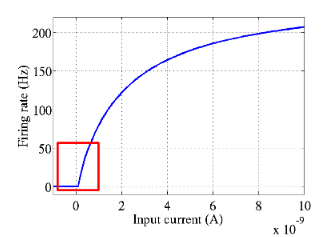
\includegraphics[width=0.6\textwidth]{biological_activation_function.png}
	\caption[Activation function inspired by biological data]{Activation function inspired by biological data\footnotemark}
	\label{fig:biological_activation_function}
\end{figure}
\footnotetext{Taken from \cite{dsrnn}, p. 3}


Another property of the \ac{ReLU}, which makes it biologically more plausible, is the fact that using the \ac{ReLU} as activation function leads to neural networks, which tend to be sparse. Sparse neural networks have only few connections or, equivalently, a lot of connections with a weight of zero. These networks are closer to natural neural networks, some of which appear to have only 1\% to 4\% of their neurons activated. On the one hand, sparse neural networks work well on naturally sparse data, on the other hand, a too sparse network may lose a lot of its modeling capability.\\
Being biologically plausible is not necessarily essential to construct a well performing machine learning model. However, in \cite{dsrnn} several comparisons between a network with the \ac{ReLU} as activation function and other models have shown that the \ac{ReLU} network performs better than the other models or is at least competitive. The \acp{CNN} used in this thesis often use combinations of the sigmoidal activation function and the \ac{ReLU}.

\subsection{Feed-forward Neural Networks}
\label{subsec:feed_forward_neural_networks}

The still most common \acp{ANN} are feed-forward neural networks. The neurons in a feed-forward neural network are usually organized in consecutive layers, which propagate the information in only one direction through the network. Figure \ref{fig:ffnn} shows a fully connected feed-forward network with one input layer, one output layer and two layers in between, which are called hidden layers.
\begin{figure}[htbp]
	\centering
	\begin{tikzpicture}[scale=1,every path/.style={>=latex}]
		%draw text nodes
		\node at (0,4.4) {Input Layer};
		\node at (9,4.9) {Output Layer};
		\node at (4.5,5.2) {Hidden Layers};
		% draw first layer
		\foreach \x in {1,...,3}
		{
			\node (n0\x) at (0, \x) [circle,draw,minimum size=0.5cm] {};
		}
		%draw second layer
		\foreach \x in {0,...,4}
     	{
     		\node (n3\x) at (3, \x) [circle,draw,minimum size=0.5cm] {};
     		% draw connections from layer one to layer two
     		\foreach \n in {1,...,3}
     		{
     			\draw[->] (n0\n) to (n3\x);
     		}
     	}
     	%draw third layer
		\foreach \x in {0,...,5}
     	{
     		\node (n6\x) at (6, \x - 0.5) [circle,draw,minimum size=0.5cm] {};
     		% draw connections from layer two to layer three
     		\foreach \n in {0,...,4}
     		{
     			\draw[->] (n3\n) to (n6\x);
     		}
     	}
     	%draw fourth layer
     	\foreach \x in {1,...,4}
     	{
     		\node (n9\x) at (9, \x - 0.5)  [circle,draw,minimum size=0.5cm] {};
     		% draw connections from layer three to layer four
     		\foreach \n in {0,...,5}
     		{
     			\draw[->] (n6\n) to (n9\x);
     		}
     	}
	\end{tikzpicture}
	\caption{Fully connected feed-forward neural network with two hidden layers}
	\label{fig:ffnn}
\end{figure}


As illustrated by the arrows in figure \ref{fig:ffnn}, the information is passed from the leftmost neurons in the input layer to the first hidden layer, then to the second hidden layer and finally to the output layer on the right. The number of neurons in the input layer has to correspond to the dimensionality of the input space. The number of neurons in the output layer is determined by the number of classes in a classification task or the number of desired outputs in a regression task respectively. Hence, these parameters are clearly defined by the problem and are not subject to the optimization process. On the other hand, the number of the neurons in the hidden layers and the number of the hidden layers itself depends on the complexity of the task, which shall be solved by the network. For easily solvable problems only a few neurons may suffice, while difficult tasks can require several hundred or thousand neurons. Figuring out an appropriate network architecture is a task, whose difficulty should be not underestimated.\\
The above depicted network is called fully-connected, because each neuron in layer $i$ has a connection to each neuron in layer $i + 1$. Note that there are no connections within one single layer. If there were also connections in the other direction, the network would be a \ac{RNN}. Although there are many interesting problems to which \acp{RNN} could be applied to, \acp{RNN} are much less prominent in Machine Learning, because there are very few well-established training algorithms. For feed-forward networks, however, exist reliable training algorithms. The most used of them is called Backpropagation. Backpropagation profits from the observation that a feed-forward \ac{ANN} is nothing more than a mathematical function, which fulfills the requirements for being differentiable. While the sigmoidal activation function and the hyperbolic tangent activation function are differentiable, the \ac{ReLU} is a bit problematic, because it is not differentiable at $0$. This problem can be eluded by setting the gradient to $0$ at this position. To understand how Backpropagation works, it is necessary to introduce an error function. The formula for a very common error function, the \ac{MSSE}, is given in equation \eqref{eq:msse}.
\label{msse}
\begin{align}
\label{eq:msse}
\operatorname{MSSE} = \frac{1}{N} \cdot \sum_{i}^{N} \left(\hat{y}_i - y_i\right)^2
\end{align}
$N$ is the number of samples, e.g. the number of images used for training an \ac{ANN}. $\hat{y}_i$ is the predicted value for the $i$-th input vector $\V{x}_i$ and $y_i$ the true value, i.e. the label, of the said input. The goal of training an \ac{ANN} is to adapt its weights such that its prediction $\hat{y}_i$ is as close as possible to the true label $y_i$. If the two values are very close, the squared difference $(\hat{y}_i - y_i)^2$ is very small and adds almost nothing to the eventual value of the sum. If the values diverge, their squared difference gets very large and the error function increases superlinearly. Thus, the \ac{MSSE} error function punishes large deviations more than small deviations.\\
The value $\hat{y}_i$ is the result of the function, which is implemented by the neural network, and therefore depends mainly on the weights. Firstly, Backpropagation calculates the gradient of the error function with respect to the weights for a subset of the input data set by applying the chain rule. Since the gradient always points in the direction of the steepest incline, the weights are adapted by subtracting the gradient multiplied with a certain value, which is called learning rate. The learning rate determines how much influence the chosen subset of input data has on the weight changes. One way to choose the mentioned data subset is to consider all data and adapt the weights after presenting all inputs to the network, i.e. calculating the prediction $\hat{y}_i$ for each input vector $\V{x}_i$. The process of presenting all inputs is called an epoch. This method has the advantage of being relatively robust against noise, because it is averaged out to a certain degree. The disadvantage is that the weights are learned rather slowly, because a lot of epochs are necessary until the network produces good results. Another method, which is called \acf{SGD}, uses only small batches, i.e. the data is divided in $n$ equally sized subsets, which are subsequently presented to the network. The idea is that the gradient of each batch is an approximation of the true gradient. Since the weights are adapted after each batch, the learning process should be faster. One possible caveat, however, is that outliers have a rather strong influence on the weight changes.\\
With $n_i$ as number of neurons in layer $i$, there are $n_i \cdot n_{i+1}$ connections between layer $i$ and layer $i+1$. That means that there are many connections, whose weights have to be learned during the training phase. Since the training time of such a network can easily last several days, more time-efficient models are desirable.

\subsection{Convolutional Neural Networks}

\acfp{CNN} are a specific kind of \acp{ANN}, which perform very well on image data, because they are able to exploit their two-dimensional structure.

\subsubsection{Convolutional Layer}
\label{subsubsec:convolutionallayer}

The key idea is to replace some of the fully connected layers at the beginning of the network with two-dimensional convolutional layers. A very important property of these layers is that they use only little weight patches, which are called filters, for the whole layer instead of connecting each neuron of one layer with all neurons of the succeeding layer. This way many connections can be omitted, resulting in a shorter training time. Figure \ref{fig:centered_filter} shows how one filter in a convolutional layer functions in general.
\begin{figure}[htbp]
	\centering
	\begin{tikzpicture}[scale=0.9,every path/.style={>=latex}]
		\node (layeri) at (2.5,11) {Layer i};
		\node (layeri) at (9.5,10) {Layer i+1};
     	
     	% draw background for filter
     	\draw[fill=pink] (2.5,2.5) rectangle (5.5,-0.5);
     	
     	% draw rectangle with "*" inside
     	\draw[fill=white] (5.2,2.8) rectangle (5.8,2.2);
     	\node at (5.5,2.5) {$*$};
     	
     	
     	% draw layer 1
     	\foreach \x in {0,...,5}
     	{
     		\foreach \y in {0,...,10}
     		{
     			\node(1-\x-\y) at (\x,\y) [circle,draw,minimum size=0.4cm] {};
     		}
     	}
     	
     	% draw layer 2
     	\foreach \x in {1,...,4}
     	{
     		\foreach \y in {1,...,9}
     		{
     			\node(2-\x-\y) at (\x + 7,\y) [circle,draw,minimum size=0.4cm] {};
     		}
     	}
     	
     	%draw filter
     	\foreach \x in {0,...,2}
     	{
     		\foreach \y in {3,...,5}
     		{
     			\node(f-\x-\y) at (\x - 0.06 + 3,\y - 0.06 - 3) [circle,draw,purple,minimum size=0.4cm] {};
     		}
     	}
     	
     	% draw line from filter to "+" rectangle
     	\draw[->] (5.5,0) to (6.7,0);
     	
     	% draw "+" rectangle
     	\draw[fill=white] (6.7,0.3) rectangle (7.3,-0.3);
     	\node at (7,0) {$+$};
     	
     	% draw line from "+" rectangle to ReLU rectangle
     	\draw[->] (7.3,0) to (8.7,0);
     	
     	% draw ReLU rectangle
     	\draw[fill=white] (8.7,0.3) rectangle (9.3,-0.3);
     	\draw[->,out=0,in=270] (9.3,0) to (2-4-1);
     	\draw[-] (8.82,-0.1) to (9.02,-0.1);
     	\draw[-] (9.02,-0.1) to (9.17,0.1);
	\end{tikzpicture}
	\caption{Functioning of a convolutional layer}
	\label{fig:centered_filter}
\end{figure}

The filter in this example has a size of $3\times 3$ and is emphasized by the 9 purple circles and by the light red background. The filter in the illustration is currently centered on the fifth neuron from the left and second from the bottom. The multiplication symbol $*$ in the small rectangle in the top right corner of the filter indicates that the activation value of each neuron, which is covered by the filter, is multiplied with the weight of the filter at the corresponding position. The resulting products are summed up to a single value, which is inserted in the activation function and finally becomes the activation of the neuron in layer $i+1$. This is done not only once, but the filter is centered on each neuron of layer $i$ in order to produce the activations of the neurons in layer $i+1$. Using this method a drastic reduction of weights is achieved by replacing the $n_i \cdot n_{i+1}$ weights, which would be required for a fully connected \ac{ANN}, with a constant number of weights, which is independent of the number of neurons in the two connected layers. The dimensionality of layer $i+1$ is slightly reduced by $(h - 1) / 2$ neurons in horizontal direction and $(v - 1)/2$ neurons in vertical direction (with $h$ = filter height and $v$ = filter width), because the filter is not centered on the outermost neurons. Edge handling techniques known from digital image processing like wrap-around or zero-padding are usually not used. The strong resemblance of the mathematical concept of convolution with the way how the filter's weights are multiplied with the activation values of the neurons is the origin of the name Convolutional Neural Network.

\subsubsection{Maps}
\label{subsubsec:maps}

Contrary to what has been suggested so far, most layers in a \ac{CNN} do not consist of only one two-dimensional array but several ones, which are called maps. A convolutional layer takes all the maps of its preceding layer as input and produces a certain amount of output maps. Figure \ref{fig:cnn_maps} illustrates in detail how such a layer works. The following lines are inspired by the explanations in \cite{gtsrb}.
\begin{figure}[htbp]
	\centering
	\begin{tikzpicture}[xscale=0.9,yscale=0.79,every path/.style={>=latex}]
		% draw input maps		
		\node (IM1) at (2,11.) [draw,rectangle,minimum width=6cm,minimum height=1.7cm] {Input map 1};
		\node (IM2) at (12,11.) [draw,rectangle,minimum width=6cm,minimum height=1.7cm] {Input map 2};
		
		% draw filters
		\node (F11) at (0,7.5) [draw,rectangle,minimum size=1cm] {$F_{11}$};
		\node (F12) at (2,7.5) [draw,rectangle,minimum size=1cm] {$F_{12}$};
		
		\node (F21) at (6,7.5) [draw,rectangle,minimum size=1cm] {$F_{21}$};
		\node (F22) at (8,7.5) [draw,rectangle,minimum size=1cm] {$F_{22}$};

		\node (F31) at (12,7.5) [draw,rectangle,minimum size=1cm] {$F_{31}$};
		\node (F32) at (14,7.5) [draw,rectangle,minimum size=1cm] {$F_{32}$};
		
		% draw lines from input maps to filters
		\draw[->] (IM1.south) to (F11.north);
		\draw[->] (IM2.south) to (F12.north);
		\draw[->] (IM1.south) to (F21.north);
		\draw[->] (IM2.south) to (F22.north);
		\draw[->] (IM1.south) to (F31.north);
		\draw[->] (IM2.south) to (F32.north);
		
		% draw convolution symbols on the filters
		\node[draw,rectangle,fill=white,above right=-0.4cm of F11] {$*$};
		\node[draw,rectangle,fill=white,above left=-0.4cm of F12] {$*$};
		\node[draw,rectangle,fill=white,above right=-0.4cm of F21] {$*$};
		\node[draw,rectangle,fill=white,above left=-0.4cm of F22] {$*$};
		\node[draw,rectangle,fill=white,above right=-0.4cm of F31] {$*$};
		\node[draw,rectangle,fill=white,above left=-0.4cm of F32] {$*$};
		
		% draw output maps
		\node (OM1) at (1,2.5) [draw,rectangle,minimum width=4cm,minimum height=1.5cm] {Output map 1};
		\node (OM2) at (7,2.5) [draw,rectangle,minimum width=4cm,minimum height=1.5cm] {Output map 2};
		\node (OM3) at (13,2.5) [draw,rectangle,minimum width=4cm,minimum height=1.5cm] {Output map 3};
		
		% draw + signs
		\node (P1) at (1,5.6) [draw,rectangle,minimum size=0.5cm] {+};
		\node (P2) at (7,5.6) [draw,rectangle,minimum size=0.5cm] {+};
		\node (P3) at (13,5.6) [draw,rectangle,minimum size=0.5cm] {+};
		
		% draw lines from filters to + signs
		\draw[->] (F11.south) to (P1.north);
		\draw[->] (F12.south) to (P1.north);
		\draw[->] (F21.south) to (P2.north);
		\draw[->] (F22.south) to (P2.north);
		\draw[->] (F31.south) to (P3.north);
		\draw[->] (F32.south) to (P3.north);

		% draw biases
		\node[draw,rectangle,left=of P1] (b1) {$b_1$};
		\node[draw,rectangle,left=of P2] (b2) {$b_2$};
		\node[draw,rectangle,left=of P3] (b3) {$b_3$};

		% draw lines from biases to + signs
		\draw[->] (b1) to (P1);
		\draw[->] (b2) to (P2);
		\draw[->] (b3) to (P3);

		% draw activation functions
		\node (A1) at (1,4.4) [draw,rectangle,minimum size=0.5cm] {};
     	\draw[-] (0.82,4.3) to (1.02,4.3) to (1.17,4.5);
		\node (A2) at (7,4.4) [draw,rectangle,minimum size=0.5cm] {};
     	\draw[-] (6.82,4.3) to (7.02,4.3) to (7.17,4.5);
		\node (A3) at (13,4.4) [draw,rectangle,minimum size=0.5cm] {};
     	\draw[-] (12.82,4.3) to (13.02,4.3) to (13.17,4.5);
		
		% draw lines from + signs to activation functions
		\draw[->] (P1) to (A1);
		\draw[->] (P2) to (A2);
		\draw[->] (P3) to (A3);

		% draw lines from activation functions to output maps
		\draw[->] (A1) to (OM1);
		\draw[->] (A2) to (OM2);
		\draw[->] (A3) to (OM3);
	\end{tikzpicture}
	\caption{How maps are organized in a convolutional layer}
	\label{fig:cnn_maps}
\end{figure}


While the very first layer of a \ac{CNN} often works on exactly three maps, each of which containing the information of one of the three color channels of an \ac{RGB} image, the convolutional layer used in the example network depicted in figure \ref{fig:cnn_maps} has only two input maps for display reasons. The number of the output maps can be chosen arbitrarily, independent of the number of the input maps. The number of the filters, on the other hand, is determined by the product of the number of the input maps and the number of the desired output maps. Hence, the network given in the illustration has exactly $2 \cdot 3 = 6$ filters. The formula for output map $O_j$ is given in equation \eqref{eq:output_map} with $N$ as number of input maps and $I_i$ as $i$-th input map.
\begin{align}
\label{eq:output_map}
O_j = f \left( \sum_i^{N} I_i * F_{ji} + b_j \right)
\end{align}
In order to calculate the output map $O_j$, each input map $I_i$ is convolved with a corresponding filter $F_{ji}$ as described above around figure \ref{fig:centered_filter}. This part is indicated by $I_i * F_{ji}$ in the formula. Thus, the number of filters needed to calculate one single output map is equal to the number of given input maps $N$. All the resulting outputs of the convolutions are summed up to one single two-dimensional array. Subsequently a scalar bias value $b_j$ is added to each element of the current intermediate result. Before this array finally becomes the output map $O_j$, an activation function like the \ac{ReLU} is applied to each neuron.\\
Since the total number of filters in a convolutional layer equals $N \cdot J$ (with $J$ as the number of output maps) and since in general all filters used in a single convolutional layer have the same dimensionality $h \times v$, the total number of weights $\abs{W}$ is computed as shown in equation \eqref{eq:total_number_of_weights}.
\begin{align}
\label{eq:total_number_of_weights}
\abs{W} = N \cdot J \cdot h \cdot v
\end{align}
To determine the total number of free parameters in a convolutional layer, the number of bias values, which corresponds to the number of output maps $J$, has to be added to the number of the weights. Hence, a convolutional layer with 5 input maps, 8 output maps and filters of size $3\times 3$ has $5 \cdot 8 \cdot 3 \cdot 3 +  8 = 368$ trainable parameters in total.

\subsubsection{Max Pooling Layer}
\label{subsubsec:maxpoolinglayer}

Next to the convolutional layer there is another layer, which is normally part of a \ac{CNN}, namely the max pooling layer. This sort of layer is used to increase the translation invariance and thus to decrease the locality of the network by combining a patch of neurons in an input map to only one neuron in an output map. This is done by choosing the maximum activation of the contemplated neurons as output. It is very common to use a $2\times 2$ patch, but also larger patches are possible. The considered neuron patches in the input map may overlap, but usually only distinct patches are regarded. Figure \ref{fig:max_pooling} illustrates this concept for a single max pooling operation on a batch of 4 neurons without overlap.
\begin{figure}[htbp]
	\centering
	\begin{tikzpicture}[scale=0.85,every path/.style={>=latex}]
		\node (layeri) at (2.5,8) {map in layer i};
		\node (layeri) at (9,5.5) {map in layer i+1};
	
     	% draw background for max pooling
     	\draw[fill=pink] (3.5,-0.5) rectangle (5.5,1.5);
     	
     	% draw left layer
     	\foreach \x in {0,...,5}
     	{
     		\foreach \y in {0,...,7}
     		{
     			\node(1-\x-\y) at (\x,\y) [circle,draw,minimum size=0.4cm] {};
     		}
     	}
     	
     	% draw right layer
     	\foreach \x in {0,...,2}
     	{
     		\foreach \y in {0,...,3}
     		{
     			\node(2-\x-\y) at (\x + 8,\y + 1.5) [circle,draw,minimum size=0.4cm] {};
     		}
     	}
     	
     	% draw "+" rectangle
     	\node (max) at (8.5,0.5) [draw,rectangle] {max};
     	
     	% draw line from red rectangle to max
     	\draw[->] (5.5,0.5) to (max);
     	
     	% draw line from max to corresponding neuron in layer i+1
     	\draw[->,out=0,in=270] (max) to (2-2-0);
	\end{tikzpicture}
	\caption{Max Pooling layer}
	\label{fig:max_pooling}
\end{figure}

As depicted in the figure, max pooling drastically decreases the number of neurons by a factor $h$ in horizontal direction and a factor $v$ in vertical direction, given a max pooling patch size of $h\times v$ and no overlap. As opposed to the convolutional layers, the max pooling layer neither combines several input maps into one output map nor produces more output maps than input maps, but generates exactly one output map for each input map instead. Thus, a max pooling layer can be used for complexity reductions only.\\
While the early layers in the network respond to basic features like edges and corners, the later layers in the network, which survey a relatively large area of the image because of the max pooling operation, respond to more complex compound features without having knowledge of the precise locations of all their contributing individual parts. This behavior is desirable particularly for classification tasks, because it is often not necessary to know in detail where the features are located in the image. In regression tasks, however, precise knowledge about the features' position is very valuable, so the use of max pooling should be left out or at least be limited to a certain degree.\\%TODO Add source
Most \acp{CNN} use convolutional layers and max pooling layers alternately, producing more and more high-level feature extractors with increasing depth of the network. After the convolutional and max pooling layers a small number of fully connected layers follows to connect the responses of the high-level feature extractors logically in order to produce reasonable predictions. The first fully connected layer has one connection to each neuron of each map of the last preceding layer. Since \acp{CNN} often possess very many consecutive layers, the network becomes very deep. This is where the recently often used terms \q{Deep Learning} and \q{Deep Convolutional Network} originate from. The layers introduced in this subsection are important components of the \acp{CNN} which are used in this thesis in order to construct an as good as possible estimator for facial landmarks in images of human faces.
\newpage

%%%%%%%%%%%%%%%%%%%%%%%%%%%%%%%%%%%%%%%%%%%%%%%%%%%%%%%%%%%%%%%%%%%%%%%%%%%%%%%%%%%%%%%%%%%%%%%%%%%%%%%%%
%%%%%%%%%%%%%%%%%%%%%%%%%%%%%%%%%%%%%%%%%%%%%%%%%%%%%%%%%%%%%%%%%%%%%%%%%%%%%%%%%%%%%%%%%%%%%%%%%%%%%%%%%
%									DATA CHAPTER BEGINS HERE											%
%%%%%%%%%%%%%%%%%%%%%%%%%%%%%%%%%%%%%%%%%%%%%%%%%%%%%%%%%%%%%%%%%%%%%%%%%%%%%%%%%%%%%%%%%%%%%%%%%%%%%%%%%
%%%%%%%%%%%%%%%%%%%%%%%%%%%%%%%%%%%%%%%%%%%%%%%%%%%%%%%%%%%%%%%%%%%%%%%%%%%%%%%%%%%%%%%%%%%%%%%%%%%%%%%%%

\section{Data}
\label{sec:data}

Training and testing a \ac{CNN} requires an appropriate data set with a sufficiently large number of training and test examples. Daniel Nouri uses the data set from the \emph{Facial Keypoints Detection} challenge on the machine learning website Kaggle (cf. \cite{kaggle}) in his inspiring tutorial \emph{Using convolutional neural nets to detect facial keypoints} \cite{nouri-tutorial}. This dataset provides a reasonable amount of landmarks, however, it does not provide all landmarks for all faces. To avoid too much data organization overhead it was used the \ac{MUCT} data set taken from \cite{muct} instead, which exhibits a simpler data structure and furnishes not only the same types of landmarks, which uses Kaggle, but even more for each depicted person.

\subsection{Kaggle}

Since the first experiments done in the scope of this thesis were inspired by the tutorial by Daniel Nouri mentioned above, it was initially planned to work with the same data set, which was used there. The data set used in the tutorial is taken from the \emph{Facial Keypoints Detection} challenge on Kaggle and contains 7049 training images as well as 1783 test images with a resolution of $96 \times 96$ pixels. All images are provided as gray value images within the range $[0,255]$.\\
There are 15 different landmarks (called keypoints on Kaggle), each of which consists of two scalar values $(x,y)$, which represent the horizontal and vertical position of the corresponding feature in the image. The 15 landmarks are:
\vspace{-0.2cm}
\begin{multicols}{2}
	\begin{itemize}[itemsep=-2ex]
		\item Left eye center
		\item Right eye center
		\item Left eye inner corner
		\item Left eye outer corner
		\item Right eye inner corner
		\item Right eye outer corner
		\item Left eyebrow inner end
		\item Left eyebrow outer end
	\end{itemize}
\columnbreak
	\begin{itemize}[itemsep=-2ex]
		\item Right eyebrow inner end
		\item Right eyebrow outer end
		\item Nose tip
		\item Mouth left corner
		\item Mouth right corner
		\item Mouth center top lip
		\item Mouth center bottom lip
	\end{itemize}
	\vphantom{}
\end{multicols}
%TODO Insert image which shows all the landmarks
\vspace{-0.5cm}
One difficulty of this data set is that not all landmarks exist for all images. In fact, for virtually each landmark exists a different set of images, which contain the landmark. This leads to problems, because a \ac{CNN} expects a fixed number of inputs and produces a fixed number of outputs. There are several ways to deal with this problem. One of them is to train a separate predictor for each landmark with all images, which contain information about the regarded landmark. The predictors could then be merged in order to produce values for all landmarks on the test images. Another way could be to predict always all landmarks but to modify the error function such that outputs, which belong to nonexistent landmarks, are not considered. To avoid these problems and because of the rather small image resolution of $96 \times 96$, another data set with a larger resolution of the raw images was used.

\subsection{MUCT Face Database}

The \acf{MUCT} face database was created by Stephen Milborrow, John Morkel and Fred Nicolls in December 2008 at the University Of Cape Town (cf. \cite{muct}). It contains 3755 faces with 76 manually set landmarks, including all Kaggle landmarks presented above. As shown in figure \ref{fig:muctfaces}, it provides a broad spectrum of faces from people of different age, gender and ethnicity. Furthermore, many different lighting settings have been used in order to increase the diversity of the pictures.

\begin{figure}[htbp]
	\centering
	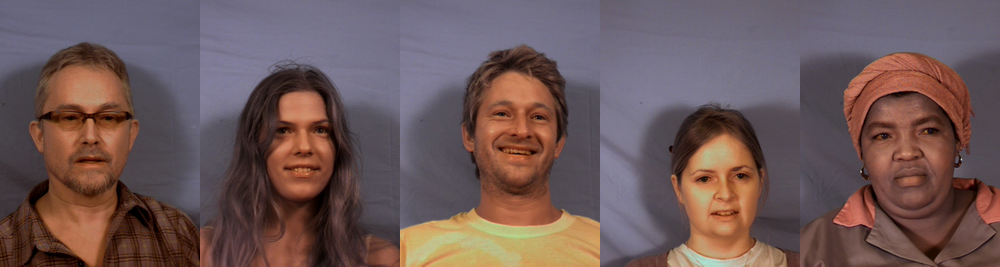
\includegraphics[width=\textwidth]{muct_faces.png}
	\caption{Five faces from the MUCT Face Database}
	\label{fig:muctfaces}
\end{figure}

Since images given in real applications are often not taken from a perfectly frontal perspective on the face, the creators of the data set provide images taken from five different angles, which are shown in figure \ref{fig:muctangles}. Disregarding some negligible software induced delays, all five images were taken simultaneously in order to guarantee that the person does not move between two photo shots. Whereas two of the images show the right side of the person's face, images of the left side were not taken, because approximations of these images can be easily obtained by mirroring.

\begin{figure}[htbp]
	\centering
	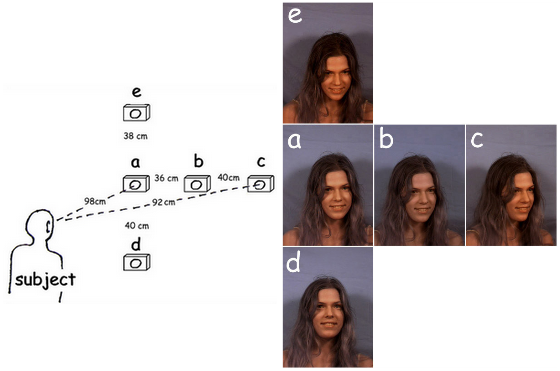
\includegraphics[width=0.77\textwidth]{muct_perspectives.png}
	\caption[MUCT Different Perspectives]{MUCT Different Perspectives\footnotemark}
	\label{fig:muctangles}
\end{figure}
\footnotetext{Both illustrations were taken from the \cite{muct} paper}

There is only one real disadvantage of the \ac{MUCT} data set compared to the Kaggle data set, namely the smaller total number of images -- 3755 on \ac{MUCT} instead of 8832 on Kaggle. Apart from that, using the \ac{MUCT} data set has a lot of advantages. The first one is the larger resolution: the \ac{MUCT} images are made available in a resolution of $480 \times 640$ pixels, whereas the Kaggle images have a resolution of only $96 \times 96$ pixels. Even if the full resolution may not be used due to execution time and memory space restrictions, larger resolutions than $96 \times 96$ allow for a model, which works more precisely with regard to rather subtle or fine landmarks. Another advantage is the accessibility of color information, which may be useful to produce reasonable predictions at the expense of a longer program execution time.\\
Another expedient property of the \ac{MUCT} data set is its well-structuredness. The file names contain all relevant information about the images, because all of them follow the pattern \texttt{i\{personID\}\{lighting setting\}\{camera view\}-\{gender\}\{(no) glasses\}}. The first \texttt{i}mage of the data set has the file name \texttt{i000qa-fn.jpg}, so the person has the ID \texttt{000}, lighting setting \texttt{q} was used, the photo was shot from angle \texttt{a}, the person is \texttt{f}emale and does \texttt{n}ot wear glasses.\\
This naming system is very comfortable, because selecting only a certain subset of the images is simplified a lot, because it is sufficient to check their filename for a specific character at the position corresponding to the chosen criterion. This is important, because also the \ac{MUCT} data set does not provide all landmarks for all images, but it does so in a much more organized and transparent way. As pointed out in \cite{muct}, it occurs only for the camera views \texttt{b} and \texttt{c} that some landmarks may not be given, because some of them are not visible due to the perspective on the face. For example the end of a person's left eyebrow is often not visible.\\
Since \acp{ANN} usually require a fixed input size and a fixed output size, all images taken from camera view \texttt{b} and \texttt{c} were omitted and not used at all. For that reason the total number of images shrinks to 2257. These images were divided randomly in 1752 training images and 502 test images by declaring 20\% of the persons as test persons. No person was assigned to both training set and test set in order to increase the generalization capability of the network. Hence, the test images presented to the network always showed persons unknown to the network.
%TODO Maybe add something about the lighting settings, if there will remain too much unused space.

\subsection{Image Preprocessing}
\label{subsec:image_preprocessing}

Before the images are passed as input to the \ac{CNN} many reasonable preprocessing operations can be applied. On the one hand, the data has to be modified before the whole training process such that training time does not become too long and furthermore that not too much memory space is required. On the other hand, it is reasonable to increase the amount of training data artificially in order to increase the network's generalization ability by distorting the training images a little bit before each epoch.

\subsubsection{Pre-Training Operations}

There are some operations, which for several reasons are applied to the training images before the training process itself starts. An important operation is the downscaling of the images, because images with a large resolution like $480\times 640$ pixels cause very long training times. Therefore it is necessary to renounce a lot of the information by rescaling the images to resolutions like $96\times 128$ or $120\times 160$ pixels.\\
Another possibility to reduce the training time and the memory space demands is to dismiss the color information by transforming the \ac{RGB} images to gray-value images. Since the number of the input maps of the first layer of the \ac{CNN} shrinks from 3 to 1, the network can be trained faster. Additionally the information passed to the network can be increased by using larger resolutions for the input images, because gray-value images do not require as much memory space as \ac{RGB} images. The experiments will show whether the color information or the larger resolution is more valuable.\\
The \ac{PIL} provides many useful image transformation methods. One of them is the \texttt{PIL.ImageOps autocontrast} method, which maximizes the contrast in the image by mapping the darkest pixel of the image to $0$ and the lightest pixel to $255$. The goal of applying this method is to simplify the learning task of the network by using the whole possible range of gray-values. This way the network does not have to try to extract information from a much smaller gray-value range than necessary, allowing for less sophisticated weights and therefore ideally for less epochs of training. Figure \ref{fig:autocontrast} shows the difference between an unmodified gray-value image from the \ac{MUCT} data set and its counterpart with maximal contrast.

\begin{figure}[htbp]
	\centering
	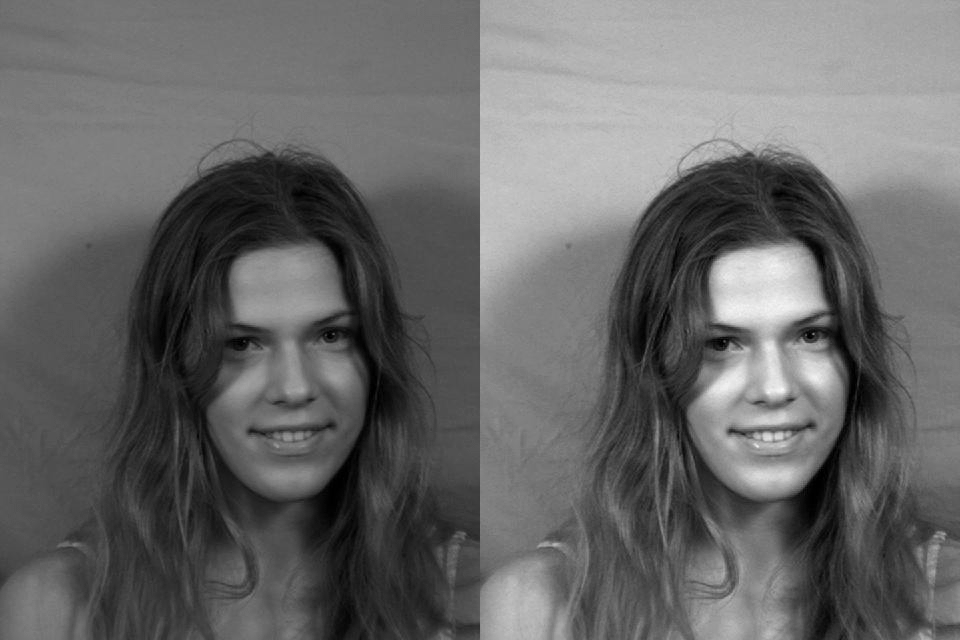
\includegraphics[width=0.5\textwidth]{gray_autocontrast.png}
	\caption{Gray-value (left) and Autocontrast (right)}
	\label{fig:autocontrast}
\end{figure}

After applying the \texttt{autocontrast} method, the gray-values of the image are normalized to the interval $[-1,1]$. The labels (i.e. the landmarks), however, are normalized to the interval $[0,1]$. Since the activation functions used in the network are zero-centered (sigmoidal function) or change their behavior at 0 (\ac{ReLU}) and since the weights of the layers are usually initialized around 0, it is reasonable to prevent that the activation functions saturates by rescaling the gray-values such that they are in the same range.\\
%TODO Maybe say that one could use a face detector before passing the images to the network.

\subsubsection{On-line Distortions}

One frequent problem of machine learning is the limited amount of training data. In order to enlarge the distribution from which the training examples are drawn and therefore to increase the generalization ability of the network, it is reasonable to produce more training examples by slightly distorting the already existing ones. Fortunately, there are many operations which can be applied to images without changing them too much. The three operations, which are applied to the images in this thesis, are translation, scaling and rotation. Throughout the whole training process these three operations are applied to each original training image before each epoch. Hence, the network sees slightly different versions of the original training images in every epoch, so that it learns a lot of possible postures of the head, even though the heads are still always from the same persons. A way to avoid that both the original images and the currently used images have to be kept in the memory is to produce the distorted images batch-wise, i.e. a small amount of images is created and passed to the network repeatedly. The used batches can be deleted immediately after having been used.\\
The first operation, which is applied to the image, is a horizontal and a vertical shift. The exact number of pixels by which an image is shifted is drawn randomly from a uniform distribution within the interval $[-0.2w, 0.2w]$ in horizontal direction and $[-0.2h, 0.2h]$ in vertical direction with $w$ as width of the image and $h$ as height of the image. Both translations are executed independently from each other and each image is shifted by an individual number of pixels. While the area of the original image, which is shifted outside of the allowed region, is discarded, the pixels, which become free after the translation, are filled with the color value of the closest pixel of the shifted image. The purpose of this operation is to increase the translation invariance of the network. Figure \ref{fig:autocontrast_shifted} shows the image from figure \myref{fig:autocontrast} shifted to the right by 10\% and down by 7\% of the image's width and height respectively.

\begin{figure}[htbp]
	\centering
	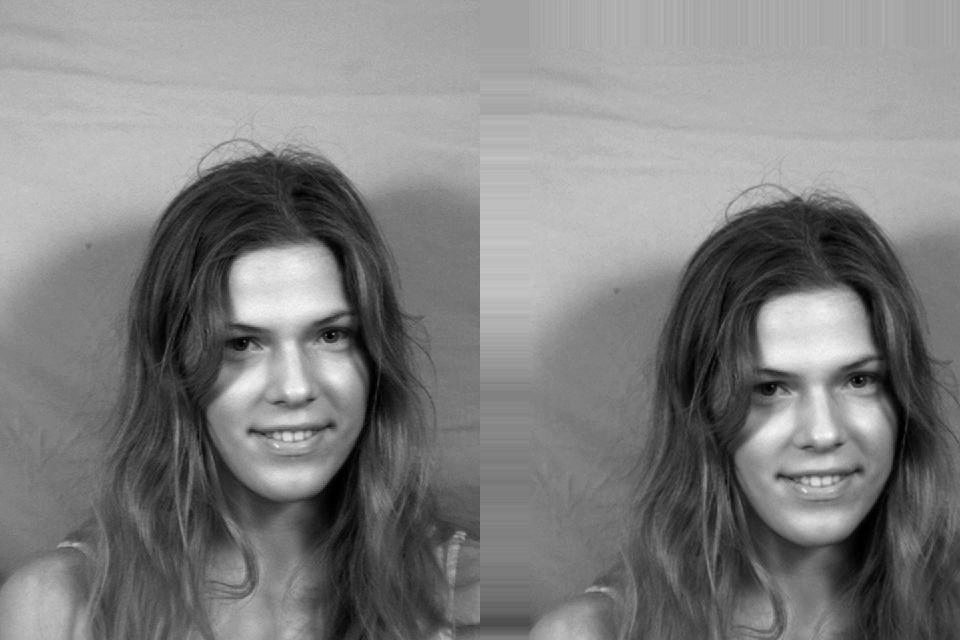
\includegraphics[width=0.5\textwidth]{autcontrast_shifted.png}
	\caption{Autocontrast (left) and Shifted (right)}
	\label{fig:autocontrast_shifted}
\end{figure}

After the translation a clockwise rotation by a degree drawn randomly for each image from the interval $[-5,5]$ follows. The corners of the image, which are rotated out of the allowed region, are discarded and the free pixels are filled with the value of the closest pixel of the rotated image. By rotating the images, the network is trained to deal images, which show persons with oblique head postures. Figure \ref{fig:shifted_rotated} shows the shifted image rotated anti-clockwise by 5\%.

\begin{figure}[htbp]
	\centering
	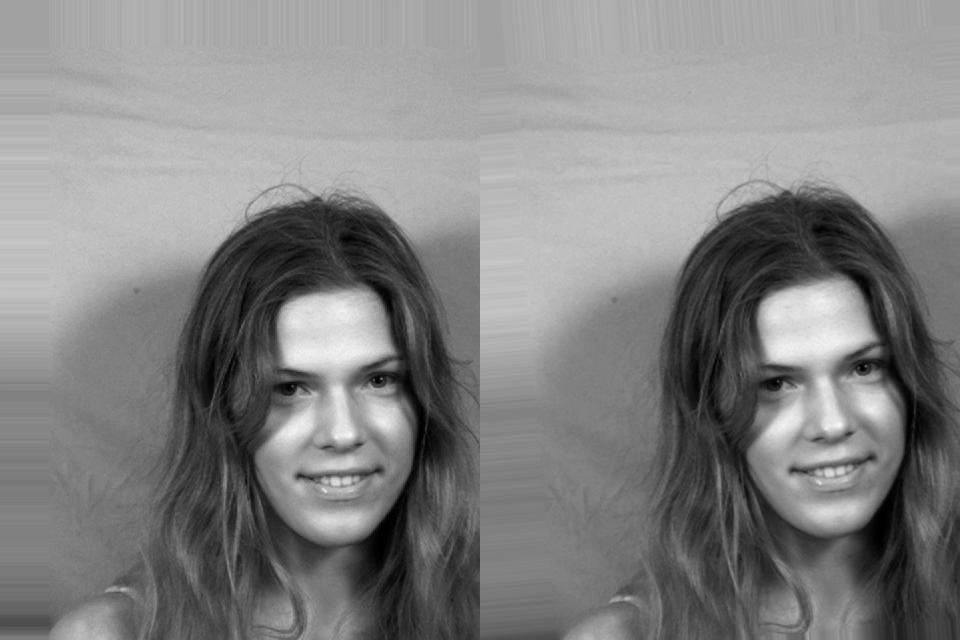
\includegraphics[width=0.5\textwidth]{shifted_rotated.png}
	\caption{Shifted (left) and Rotated (right)}
	\label{fig:shifted_rotated}
\end{figure}

Lastly, each image is scaled individually by a randomly drawn factor from the interval $[-0.95,1.05]$. If the image is enlarged all four borders are cut such that the images assumes the correct resolution. If the image is downsized, it is centered in the new image and the borders are filled with the color value of the closest pixel of the scaled image. The goal of rescaling the images is to allow different head sizes and distances of the persons from the camera. Figure \ref{fig:rotated_scaled} shows the rotated image enlarged by an unrealistically large factor of $1.2$, which was chosen in order to achieve a better visualization.

\begin{figure}[htbp]
	\centering
	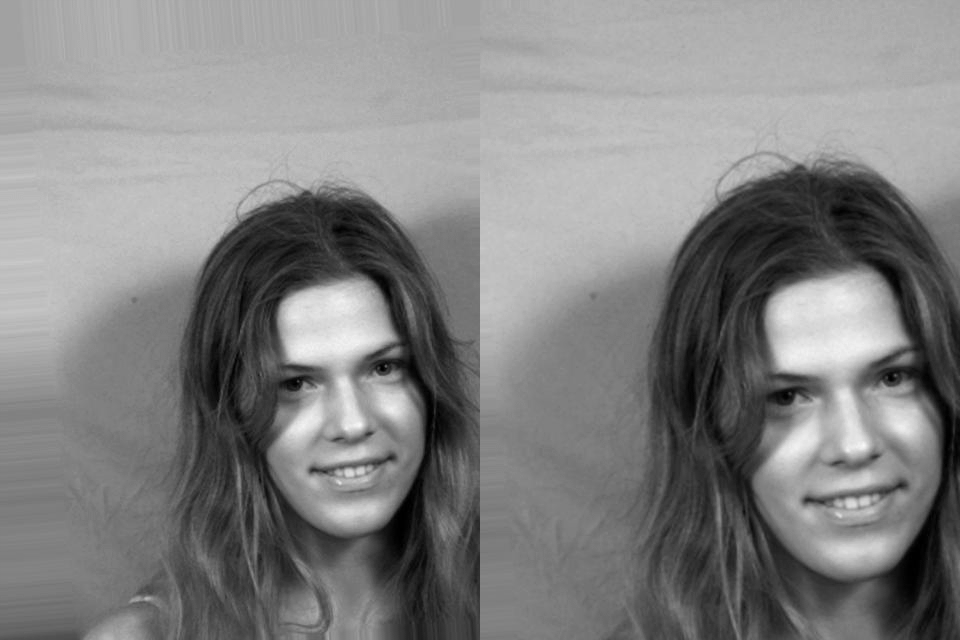
\includegraphics[width=0.5\textwidth]{rotated_scaled.png}
	\caption{Rotated (left) and Scaled (right)}
	\label{fig:rotated_scaled}
\end{figure}

\newpage

%%%%%%%%%%%%%%%%%%%%%%%%%%%%%%%%%%%%%%%%%%%%%%%%%%%%%%%%%%%%%%%%%%%%%%%%%%%%%%%%%%%%%%%%%%%%%%%%%%%%%%%%%
%%%%%%%%%%%%%%%%%%%%%%%%%%%%%%%%%%%%%%%%%%%%%%%%%%%%%%%%%%%%%%%%%%%%%%%%%%%%%%%%%%%%%%%%%%%%%%%%%%%%%%%%%
%								NETWORK ARCHITECTURES CHAPTER BEGINS HERE								%
%%%%%%%%%%%%%%%%%%%%%%%%%%%%%%%%%%%%%%%%%%%%%%%%%%%%%%%%%%%%%%%%%%%%%%%%%%%%%%%%%%%%%%%%%%%%%%%%%%%%%%%%%
%%%%%%%%%%%%%%%%%%%%%%%%%%%%%%%%%%%%%%%%%%%%%%%%%%%%%%%%%%%%%%%%%%%%%%%%%%%%%%%%%%%%%%%%%%%%%%%%%%%%%%%%%

\section{Network Architectures}
\label{sec:networkarchitectures}

Before a \ac{CNN} can be trained in order to estimate the positions of the landmarks, many decisions have to be made and a lot of parameters have to be set. On the one hand, there are fundamental decisions, which already by themselves have a considerable influence on the success or the failure of the learning process, comprising an appropriate optimization method, a suitable error function, an adequate initialization of the network's weights and the overall structure of the \ac{CNN} like the number, types and sizes of the layers. The optimization method will be the same for all investigated network configurations, namely the \ac{SGD}, which was already described in chapter \myref{subsec:feed_forward_neural_networks}. The error function will the \ac{MSSE} as described in this chapter's second subsection. The weights of the network are initialized intelligently according to the initialization method introduced by Xavier Glorot, which is described in more detail in the first subsection of this chapter. The number of used layers, their types and their sizes, however, vary from network to network and are adjusted to other parameters like the resolution of the input images.\\
On the other hand, there is large number of parameters, which require fine tuning. Some of these parameters are the learning rate, the size of the batches, which are presented successively to the network, the resolution of the input images, the usage or the disuse of the color information and the number of epochs, for which the network shall be trained. Each considered network uses different configurations for these parameters, which are always given for each described network.

\subsection{Initialization}
\label{subsec:glorot_initialization}

Early network configurations using a uniform distribution for initializing the weights of the network have not shown to be very successful. Since it is not trivial to define a reasonable range for the weights, an intelligent initialization of the weights is desirable. Xavier Glorot and Yoshua Bengio introduce such a kind of initialization in their paper \q{Understanding the difficulty of training deep feed-forward neural networks} \cite{glorotinitialization}. The authors of the paper propose the so called \emph{normalized initialization}, which sets the weights according to the formula given in equation \eqref{eq:glorotinitialization}.
\begin{align}
\label{eq:glorotinitialization}
W \sim \mathcal{U} \left[ - \frac{\sqrt{6}}{\sqrt{n_j + n_{j+1}}}, \frac{\sqrt{6}}{\sqrt{n_j + n_{j+1}}} \right]
\end{align}
$\mathcal{U}[a,b]$ is the uniform distribution in the interval from $a$ to $b$, $W$ is the weight matrix of layer $j$ and $n_i$ is the number of neurons found in layer $i$. The bias values were all set to $0$. According to the formula for the weights, the maximal absolute value of the weights between two layers is large if both layers consist of rather few neurons and vice versa.
The advantages of this initialization method are that it helps to avoid the saturation of the activation functions and that it keeps the variances of the activations and the variances of the back-propagated gradients approximately equal in all layers. This way alterations of the weights effectuated by the back-propagation do not vanish and have an actual influence on the optimization process. Next to the uniform distribution there is another initialization method often called Glorot normal initialization, which uses a normal distribution instead of a uniform distribution. It provides the same benefits as the normalized initialization but turns out to work slightly better on the problem given in this thesis than the variant with the uniform distribution. The formula is given in equation \eqref{eq:glorotinitializationnormal}. The second parameter defines the variance of the Gaussian.
\begin{align}
\label{eq:glorotinitializationnormal}
W \sim \mathcal{N} \left(0, \frac{2}{n_j + n_{j+1}} \right)
\end{align}
Even if the considerations in the mentioned paper assume the uniform distribution as well as equal sizes for all layers and were verified for dense \acp{ANN} only, they presumably work well also for different layer sizes and other network architectures like \acp{CNN}. This seems to be confirmed by the results observed in this thesis, which became significantly better after exchanging the initialization with a layer size independent uniform distribution with the Glorot normal initialization.\\

\subsection{Error Function}

All examined networks use the \ac{MSSE}, which was already explained in chapter \myref{msse} and whose formula is given in equation \eqref{eq:msse}. However, it is necessary to explain in detail how the error is calculated, because at the first glance there are at least two different theoretical possibilities. The probably most intuitive way to calculate the error is shown in figure \ref{fig:msse_landmarkwise}.
\begin{figure}[htbp]
	\centering
	
	% landmark-wise distance
	\begin{subfigure}[t]{0.5\textwidth}
		\centering
		\begin{tikzpicture}[scale=0.85,every path/.style={>=latex}]
			% draw grid
			\draw (0.5,0.5) grid (8.5,4.5);
		
			% draw nodes
			\node (E_true) at (3,2) [draw,circle,fill=AI-BLUE] {};
			\node (E_pred) at (6,3) [draw,circle,fill=yellow] {};
			\node [below=0cm of E_true] {True Label};
			\node [above=0cm of E_pred] {Prediction};
		
			% draw arrows
			\draw[<->,line width=1.5] (E_true) to (E_pred);
		\end{tikzpicture}
		\caption{Landmark-wise}
		\label{fig:msse_landmarkwise}
	\end{subfigure}
	% coordinate-wise distance
	\begin{subfigure}[t]{0.49\textwidth}
		\centering
		\begin{tikzpicture}[scale=0.85,every path/.style={>=latex}]
			% draw grid
			\draw (0.5,0.5) grid (8.5,4.5);
		
			% draw nodes
			\node (M_true) at (3,2) [draw,circle,fill=AI-BLUE] {};
			\node (M_pred) at (6,3) [draw,circle,fill=yellow] {};
			\node [below=0cm of M_true] {True Label};
			\node [above=0cm of M_pred] {Prediction};

			% draw arrows
			\draw[<->,line width=1.5] (M_true) to (6,2);
			\draw[<->,line width=1.5] (6,2) to (M_pred);
		\end{tikzpicture}
		\caption{Coordinate-wise}
		\label{fig:msse_coordinatewise}
	\end{subfigure}
	
	\caption{Two different distance measures for calculating the \ac{MSSE}}
	\label{fig:msse}
\end{figure}

This landmark-wise method adds up the squared Euclidean distances between the landmarks predicted by the network (yellow) and the true landmarks (blue). In this scenario the network seems to "know" that the $x$-coordinate and the $y$-coordinate of one landmark constitute a unit. A second possibility is shown in figure \ref{fig:msse_coordinatewise}, where the $x$-coordinate and the $y$-coordinate of a landmark are considered as two independent output values. Here both the horizontal and the vertical deviation are calculated and squared separately. Intuitively, the network should not treat a pair containing the two outputs for one landmark's coordinates differently than a pair of two arbitrarily chosen output values. However, the value produced by the error function does not change at all, no matter which way to calculate it may be chosen. This is proven by the equations \eqref{eq:equal_msse_start} - \eqref{eq:equal_msse_end}. Note that $\l_x$ is the difference between the true and the predicted $x$ value of landmark $l$.
\begin{align}
\label{eq:equal_msse_start}
\sum_{l\ \in \text{ Landmarks}} \sqrt{l_x^2 + l_y^2}^2 &= \sum_{c\ \in \text{ Coordinates}} c_x^2 + c_y^2\\
\equiv \hspace{0.3cm} \sqrt{a_x^2 + a_y^2}^2 + \sqrt{b_x^2 + b_y^2}^2 + \sqrt{c_x^2 + c_y^2}^2 &= a_x^2 + a_y^2 + b_x^2 + b_y^2 + c_x^2 + c_y^2\\
\label{eq:equal_msse_end}
\equiv \hspace{1.95cm} a_x^2 + a_y^2 + b_x^2 + b_y^2 + c_x^2 + c_y^2 &= a_x^2 + a_y^2 + b_x^2 + b_y^2 + c_x^2 + c_y^2
\end{align}
Hence, both methods are completely equivalent and since the coordinate-wise error function is easier to implement, it was used for all networks in the scope of this thesis.

The definition of the error function serves its mathematical and computational purpose, but the resulting error value is not very intuitive for human observers due to the normalization of the labels to the unit interval. The standard way of transforming the error value into a more intuitively comprehensible value is compute its square root and to multiply it with the resolution of the largest dimension of the training images. The result of this calculation is the an approximation of the average distance in pixels of the predicted labels from the true labels.

\subsection{Conventionally Trained CNN}

During the initial phase of this thesis many classical \acp{CNN} with various parameter settings have been constructed. While the purpose of this subsection is to describe the general structure of these \acp{CNN} only, the results chapter will give insight to the detailed para\-meter settings for each tested network.\\
Since it is difficult to find a suitable network architecture offhand without further knowledge or intuition, especially the networks in the early stages of this thesis are very similar to those, which were used in Daniel Nouri's tutorial \cite{nouri-tutorial}. Figure \ref{fig:example_cnn} shows a possible example network with 2 convolutional layers, each of which succeeded by a max pooling layer with a patch size of $2\times 2$. Before specifying the details of the network structure, it must be mentioned that for space saving reasons the depicted number of neurons does not correspond to the actually displayed number of neurons. In addition, the activation functions and biases were omitted for the sake of improved clarity. For the same reason there are only 2 convolutional layers instead of 3 like in \cite{nouri-tutorial}.
\begin{figure}[h!]
	\centering
	\begin{tikzpicture}[scale=0.75,every path/.style={>=latex}]%0.635%0.73
		% ========================================================================================= %
		% draw input maps
		\def\limX{0} % x-position of the leftmost input map
		\def\limY{1} % y-position of the leftmost input map
		\node at (\limX - 4, \limY + 1) {\small 3 input maps};
		
		\draw[step=0.1] (\limX,\limY) grid (\limX + 1.5,\limY + 2.0);
		\draw[step=0.1] (\limX + 2,\limY) grid (\limX + 3.5,\limY + 2.0);
		\draw[step=0.1] (\limX + 4,\limY) grid (\limX + 5.5,\limY + 2.0);
		
		% ========================================================================================= %
		% draw first convolutional and max pooling layer
		\def\lflmX{-5} % x-position of the leftmost first layer map
		\def\lflmY{-3} % y-position of the leftmost first layer map
		\node at (\lflmX - 1, \lflmY + 2.7) {\small 96 convolutional filters};
		\node at (\lflmX - 0.5, \lflmY + 0.8) {\small 32 maps};
		\node at (\lflmX - 1, \lflmY - 0.5) {\small 32 max pooling filters};
		\node at (\lflmX - 0.5, \lflmY - 1.5) {\small 32 maps};
		
		\foreach \x in {-1,0,2,3}
		{
			% draw maps of the first convolutional layer
			\draw[step=0.1] (2 * \x - 0.001,\lflmY - 0.001) grid (2* \x + 1.201,\lflmY + 1.6);
			
			% draw filters to the map
			\foreach \i in {0,...,2}
			{
				% draw filter
				\draw[step=0.1] (2 * \x + 0.4 * \i - 0.001,\lflmY + 2.5 - 0.001) grid (2* \x + 0.4 * \i + .301,\lflmY + 2.5 + .301);
				
				% draw connections from input maps to the filters
				\draw[->] (\limX + \i * 2 + 0.75,\limY) to (2 * \x + 0.4 * \i + 0.15,\lflmY + 2.5 + .301);
				
				% draw connections from filter to next map
				\draw[->] (2 * \x + 0.4 * \i + 0.15, \lflmY + 2.5 - 0.001) to (2 * \x + 0.6,\lflmY + 1.6);
			}
		
			% draw max pooling filter
			\draw[step=0.1] (2 * \x + 0.499,\lflmY - .601) grid (2* \x + .701,\lflmY - .399);
			
			% draw connection from first convolutional layer maps to max pooling filters
			\draw[->] (2* \x + 0.6,\lflmY + 1.6) to (2* \x + .6,\lflmY - .399);
			
			% draw first max pooling layer map
			\draw[step=0.1] (2 * \x + 0.199,\lflmY - 2.101) grid (2* \x + 1.001,\lflmY + -1.0);
			
			% draw connection from max pooling filter to max pooling map
			\draw[->] (2 * \x + 0.6,\lflmY - .601) to (2* \x + .6,\lflmY + -1.0);
		}
		
		% draw dots between the filters and the first layer maps
		\node at (\lflmX + 7.7, \lflmY - 1.6) {\ldots};
		\node at (\lflmX + 7.7, \lflmY - 0.5) {\ldots};
		\node at (\lflmX + 7.7, \lflmY + 0.7) {\ldots};
		\node at (\lflmX + 7.7, \lflmY + 2.65) {\ldots};
		
		% ========================================================================================= %
		% draw second convolutional and max pooling layer
		\def\lslmX{-5} % x-position of the leftmost first layer map
		\def\lslmY{-9.5} % y-position of the leftmost first layer map

		\node at (\lslmX - 3, \lslmY + 2.7) {\small 2048 convolutional filters};
		\node at (\lslmX - 2.5, \lslmY + 1.2) {\small 64 maps};
		\node at (\lslmX - 3, \lslmY + 0.1) {\small 64 max pooling filters};
		\node at (\lslmX - 2.5, \lslmY - 1.0) {\small 64 maps};
		
		\foreach \x in {-2,-1,0,2,3,4}
		{
			% draw second convolutional layer maps
			\draw[step=0.1] (2 * \x + 0.299,\lslmY + 0.799) grid (2* \x + 0.901,\lslmY + 1.6);
			
			% draw filters to the map
			\foreach \i in {-1,0,2,3}
			{
				% draw filter
				\draw[step=0.1] (2 * \x + 0.3 * \i + 0.199,\lslmY + 2.5 - 0.001) grid (2* \x + 0.3 * \i + .401,\lslmY + 2.5 + .201);
				
				% draw connections from first max pooling layer maps to the filters
				\draw[->] (2 * \i + 0.6,\lflmY - 2.101) to (2* \x + 0.3 * \i + .3,\lslmY + 2.4 + .301);
				
				% draw connections from filter to next map
				\draw[->] (2 * \x + 0.3 * \i + 0.3, \lslmY + 2.5 - 0.001) to (2 * \x + 0.6,\lslmY + 1.6);
			}
			
			% draw dots between the filters of this map
			\node at (2 * \x + 0.6,\lslmY + 2.6) {\tiny ...};
			
			% draw max pooling filter
			\draw[step=0.1] (2 * \x + 0.499,\lslmY - .001) grid (2* \x + .701,\lslmY + .201);
			
			% draw connection from second convolutional layer maps to max pooling filters
			\draw[->] (2* \x + 0.6,\lslmY + 1.6) to (2* \x + .6,\lslmY + .201);
			
			% draw second max pooling layer map
			\draw[step=0.1] (2 * \x + 0.399,\lslmY - 1.201) grid (2* \x + .801,\lslmY + -0.6);
			
			% draw connection from max pooling filter to max pooling map
			\draw[->] (2 * \x + 0.6,\lslmY + .201) to (2* \x + .6,\lslmY + -0.6);
		}
		
		% draw dots between the filters and the first layer maps
		\node at (\lslmX + 7.7, \lslmY + 0.15) {\ldots};
		\node at (\lslmX + 7.7, \lslmY - 0.9) {\ldots};
		\node at (\lslmX + 7.7, \lslmY + 1.2) {\ldots};
		\node at (\lslmX + 7.7, \lslmY + 2.65) {\ldots};
		
		% ========================================================================================= %
		% draw first fully connected layer
		\def\lffclX{-4} % leftmost x-position of the first fully connected layer
		\def\rffclX{9} % rightmost x-position of the first fully connected layer
		\def\ffclY{-13} % y-position of the first fully connected layer
		\node at (\lffclX - 3,\ffclY) {\small 500 neurons};
		
		\foreach \x in {\lffclX,...,\rffclX}
		{
			\node (n\x) at (\x,\ffclY) [draw,circle,inner sep=0pt,minimum size = 0.2cm] {};
			
			\foreach \a in {-2,-1,0,2,3,4}
			{
				\draw[->] (2 * \a + 0.599,\lslmY - 1.201) to (n\x);
			}
		}
		
		% ========================================================================================= %
		% draw second fully connected layer
		\def\lsfclX{-3} % leftmost x-position of the second fully connected layer
		\def\rsfclX{8} % rightmost x-position of the second fully connected layer
		\def\sfclY{-15.} % y-position of the second fully connected layer
		\node at (\lsfclX - 3,\sfclY) {\small 400 neurons};
		
		\foreach \x in {\lsfclX,...,\rsfclX}
		{
			\node (m\x) at (\x,\sfclY) [draw,circle,inner sep=0pt,minimum size = 0.2cm] {};
			
			\foreach \a in {\lffclX,...,\rffclX}
			{
				\draw[->] (n\a) to (m\x);
			}
		}
		
		% ========================================================================================= %
		% draw output layer
		\def\lolX{1} % leftmost x-position of the output layer
		\def\rolX{3} % rightmost x-position of the output layer
		\def\olY{-17.} % y-position of the output layer
		\node at (\lolX - 5,\olY) {\small 30 output neurons};
		
		\foreach \x in {\lolX,...,\rolX}
		{
			\node (q\x) at (\x + 0.5,\olY) [draw,circle,inner sep=0pt,minimum size = 0.2cm] {};
			
			\foreach \a in {\lsfclX,...,\rsfclX}
			{
				\draw[->] (m\a) to (q\x);
			}
		}
	\end{tikzpicture}
	\caption{A complete example \ac{CNN}}
	\label{fig:example_cnn}
\end{figure}
\\
It is assumed that the network takes \ac{RGB} images, hence there are 3 input maps, one for each color channel. The first convolutional layer is supposed to produce 32 output maps, hence according to the explanations in chapter \myref{subsubsec:maps} there are 96 filters between the input layer and the first convolutional layer. As indicated in the figure, the resulting 32 output maps of the first convolutional layer are a bit smaller in both dimensions, because the edges of the input maps are not treated. The 32 output maps of the first convolutional layer constitute the input of the first max pooling layer, which reduces the dimensionality of the maps by a factor of 2 in both dimensions. The second convolutional layer generates 64 output maps, thus $32 \cdot 64 = 2048$ filters are necessary to execute the convolution operation. Also these 64 resulting slightly smaller maps are max pooled, yielding 64 significantly smaller maps. After the second max pooling operation, two fully connected layers follow. Each neuron in the 64 output maps of the second max pooling layer has a connection to each neuron in the first fully connected layer. Assuming a resolution of $22\times 30$ in the 64 max pooling maps and 500 neurons in the first fully connected layer, there are $22 \cdot 30 \cdot 64 \cdot 500 = 21.120.000$ connections, which have to be trained. The second fully layer in this example consists of 400 neurons, thus there are $500 \cdot 400 = 200.000$ connections between the 2 fully connected layers. The last layer of the network is the output layer, which has as many neurons as there exist desired output values. In the landmark estimation task examined in this thesis the number of output neurons equals 30, because the networks were usually trained to predict the $x$-coordinate and the $y$-coordinate of 15 landmarks.\\
Even if the details will be different for each of the actually trained networks, which are presented in the results chapter, this example network should give a visual intuition for the qualitative structure of a \ac{CNN}. In the results chapter there will be detailed information about the used layer types, layer sizes, weight initializations, activation functions, learning rates and every other important parameter.

\subsection{Gabor CNNs}
\label{subsec:gaborcnns}

After training various conventional \acp{CNN} another biologically inspired kind of \ac{CNN} was constructed and tested in several different configurations. In biology there are various kinds of cells involved in the process of vision. The simple cells in the primary visual cortex detect very elementary features like corners and edges and propagate forward their output to the complex cells, which for their part are high-level feature extractors. They receive input from several simple cells and combine them in order to detect more complex features composed of simpler elements. \acp{CNN} behave similarly as the filters of the early layers resemble simple cells and the filters in the deeper layers can be considered complex cells. So far all weights of the network were trained during the learning process. The idea of the networks presented in this subsection is to refrain from training the weights of the filters of the first convolutional layer and to replace them with biologically inspired filters, which are known to work well on image data. According to \cite{ebgm} Gabor wavelets are regarded a suitable model of the simple cells, thus, they might be an adequate choice for being set as filters in the first convolutional layer. Before describing in detail the structure of the used networks, it is necessary to introduce the Gabor wavelets mathematically. They were computed according to formula \eqref{eq:gabor_wavelet}, which is taken from \cite{ebgm}.
\begin{align}
\label{eq:gabor_wavelet}
\psi_{\vec{k}}(\vec{x}) = \frac{\vec{k}}{\sigma^2} \cdot \exp\left(-\frac{\vec{k}^2\vec{x}^2}{2\sigma^2}\right) \cdot \left(\exp\left(i\vec{k}\vec{x}\right) - \exp\left(-\frac{\sigma^2}{2}\right)\right)
\end{align}
The formula contains three exponential functions, the first of which is a Gaussian, whose width is defined by $\frac{\sigma}{k}$. Euler's formula states that $\exp(ix) = \cos x + i \sin x$, hence the second exponential makes the whole function complex. Its real part is determined by a cosine-wave and the imaginary part by a sine-wave, vector $\vec{k}$ in the argument of the exponential function defines the spatial frequency (and therefore the width) and the orientation of the waves. The third exponential function corrects the wavelet such that it has zero mean, while the factor at the beginning of the formula ensures the normalization of the wavelet. An important property of the here defined wavelets is that for a fixed $\sigma$ they are identical versions of each other apart from scaling and rotation, which are defined by $\vec{k}$.\\
Formula \eqref{eq:gabor_wavelet} describes a continuous version of the Gabor wavelets. Since the Gabor wavelets shall be used in a computer model, it is necessary to discretize them. The wavelets themselves are discretized by means of the image resolution, whereas wave vector $\vec{k}$ is calculated for a chosen subset of widths and frequencies as shown in equation \eqref{eq:k}. 
\begin{align}
\label{eq:k}
\vec{k}_{m,l} = k_\text{max} \alpha^{-m} \begin{pmatrix}\cos\left(\frac{\pi l}{L}\right)\\ \sin\left(\frac{\pi l}{L}\right)\end{pmatrix} \quad m = 0, \ldots, M - 1, \quad l = 0, \ldots, L-1
\end{align}
The variable $L$ defines the number of orientations, while the variable $M$ determines the number of frequencies. \cite{ebgm} recommends specific values for each of the variables except for $k_\text{max}$. While $k_\text{max}$ was set to $\frac{\pi}{2}$, the other values were copied from \cite{ebgm}. Hence, all Gabor wavelets created in this thesis use the following parameter configuration: $\alpha = \sqrt{2}$, $\sigma = 2\pi$, $L = 8$ and $M = 5$. Thus, there are 8 orientations and 5 frequencies, yielding 40 filters each with a real part and an imaginary part. Figure \ref{fig:gabor_filters} illustrates the real parts of the 40 resulting filters. Since the imaginary parts are solely slightly phase-shifted but look otherwise  exactly like the real parts, they were omitted in the figure.
\begin{figure}[htbp]
	\centering
	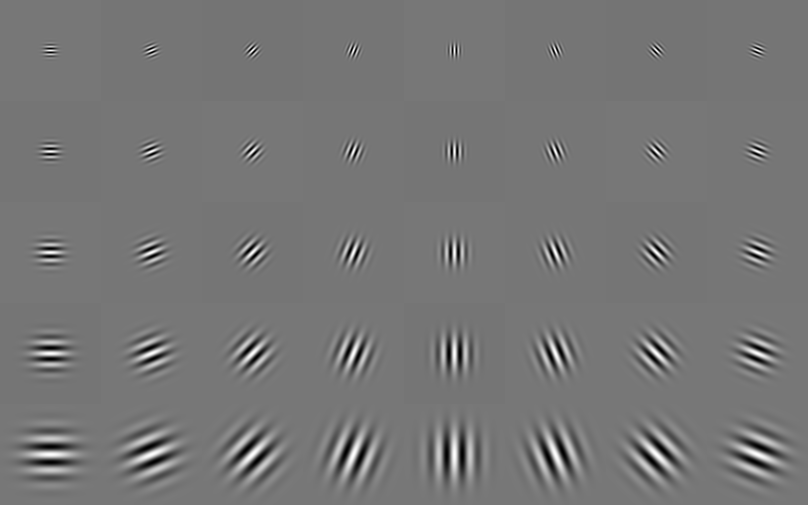
\includegraphics[width=\textwidth]{gabor_filters_normalized_filterwise_real.png}
	\caption{40 gabor filters with 8 different orientations and 5 different widths}
	\label{fig:gabor_filters}
\end{figure}\\
The filters depicted in the figure all have a size of $101 \times 101$. The size of the filters used in the \acp{CNN}, however, was reduced by cutting off the area around the wavelets, which contains only values smaller than $10^{-3}$. Since there are 5 different spatial frequencies, there are also 5 different filter sizes, namely $27 \times 27$ for $M = 0$, $31 \times 31$ for $M = 1$, $39 \times 39$ for $M = 2$, $47 \times 47$ for $M = 3$ and finally $55 \times 55$ for $M = 4$. This has the two advantages of reducing the computation time and avoiding convolutions of the input images with filter values so close to 0 that the results contain almost no information. Figure \ref{fig:gabor_filter_sizes} shows the actually used areas of the filters for $L=0$ and $M \in \{0,\ldots,4\}$. All values, which are not inside the red square, are omitted.
\begin{figure}[htbp]
	\centering
	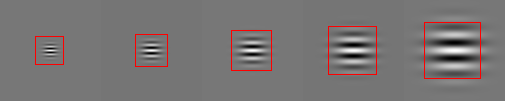
\includegraphics[width=\textwidth]{gabor_filter_sizes.png}
	\caption{The 5 actual filter sizes for $L=0$ and $M \in \{0,\ldots,4\}$}
	\label{fig:gabor_filter_sizes}
\end{figure}

\subsubsection{Gabor Layer}
\label{subsubsec:gaborlayer}

After creating the digital versions of the Gabor wavelets, they have to be incorporated in a \ac{CNN}. It was already mentioned that the filters of the first convolutional layer will be replaced with the Gabor wavelets. However, there are still many open questions about the detailed structure of this first layer, the way how to further process the responses of the wavelets and how to construct the overall structure of the \ac{CNN}. Firstly, the structure of the first convolutional layer, which will be called Gabor layer from now on, will be examined in detail. The Gabor layer itself actually consists of two layers, one of them containing the real parts and one of them the imaginary parts of the Gabor filters. The exact number of filters depends on whether color information is used or not. If the network relies on gray-values only, there are exactly 40 real filters and 40 imaginary filters (with $L = 8$ and $M = 5$). Figure \ref{fig:merge_real_imag} illustrates how the Gabor layer is organized.

\begin{figure}[htbp]
	\centering
	\newcommand\sfMergeRealImag{0.9}
	\newcommand\gridnode[5]{
		\node (#1) at (#2 + #4 / 2,#3 + #5 / 2) [minimum width=#4cm * \sfMergeRealImag,minimum height=#5cm * \sfMergeRealImag] {};
		\draw[step=0.1] (#2 - 0.001,#3 - 0.001) grid (#2+#4 + 0.001,#3+#5 + 0.001);	
	}
	\begin{tikzpicture}[scale=\sfMergeRealImag,every path/.style={>=latex}]
		% draw input image
		\gridnode{inputimage}{7.7}{3}{1.5}{2}
	
		% draw background boxes
		\draw[fill=lightgray] (0,1.5) rectangle (8,-0.5);
		\draw[fill=lightgray] (9,1.5) rectangle (17,-0.5);
	
		% draw real filters
		\foreach \x in {0,...,3}
		{
			\gridnode{r\x}{\x * 2 + 0.5}{0}{1}{1}
			\node at (\x * 2 + .5, 1) [draw,fill=white] {$*$};
			\draw[->] (inputimage.south) to (r\x.north);
			\node (ar\x) at (\x * 2 + 1., -1.3) [draw,rectangle,minimum size=0.5cm] {};
			\draw[-] (\x * 2 + 0.85, -1.4) to (\x * 2 + 1.05,-1.4) to (\x * 2 + 1.15, -1.2);
			\draw[->] (r\x.south) to (ar\x.north);
		}
		
		% draw imaginary filters
		\foreach \x in {0,...,3}
		{
			\gridnode{i\x}{\x * 2 + 9.5}{0}{1}{1}
			\node at (\x * 2 + 10.5, 1) [draw,fill=white] {$*$};
			\draw[->] (inputimage.south) to (i\x.north);
			\node (ai\x) at (\x * 2 + 10., -1.3) [draw,rectangle,minimum size=0.5cm] {};
			\draw[-] (\x * 2 + 9.85, -1.4) to (\x * 2 + 10.05,-1.4) to (\x * 2 + 10.15, -1.2);
			\draw[->] (i\x.south) to (ai\x.north);
		}
		
		% draw merge operators
		\foreach \x in {0,...,3}
		{
			\node (m\x) at (\x * 3 + 4,-3.5) [draw,rectangle] {merge op};
			\draw[->] (ar\x.south) to (m\x.north);
			\draw[->] (ai\x.south) to (m\x.north);
		}
		
		% draw output maps
		\foreach \x in {0,...,3}
		{
			\gridnode{o\x}{\x * 3 + 3.4}{-6.6}{1.2}{1.6}
			\draw[->] (m\x.south) to (o\x.north);
		}
		
		% draw text nodes
		\node at (6,4) {Input image};
		\node at (4,2.5) {40 real filters};
		\node at (13.5,2.5) {40 imaginary filters};
		\node at (1.5,-3.5) {Merging};
		\node at (1.55,-6.) {40 output maps};
	\end{tikzpicture}
	\caption{Merging the real and the imaginary filters}
	\label{fig:merge_real_imag}
\end{figure}


The very top of the figure shows the input image, consisting of only one map due to the refusal of the color information. Below there are depicted four of the forty real filters on the left and four of the forty imaginary filters on the right. The input map is convolved with each of these 80 filters, resulting in 40 real output maps and 40 imaginary output maps. Then, these 80 output maps are inserted into an activation function like the \ac{ReLU}. Afterwards, the output map of the real filter and the output map of the imaginary filter, which originally belonged to one single Gabor filter, are merged as illustrated by the small rectangle containing the text \q{merge op}. The result of the individual merging operations are 40 output maps, which will become the input of a subsequent layer. If the color information were included into the calculation, there would be 3 input maps instead of 1. The only other difference is that 240 instead of 80 filters would be used. Since each color channel should be convolved with the same values, each of the 80 filters would be used 3 times. As illustrated by figure \myref{fig:cnn_maps}, the responses of the three filters would be added up and inserted into the activation function. Independent of whether the color information is used or not, there exists one bias value for each filter. These values were omitted in figure \ref{fig:merge_real_imag} in order to keep the figure as clearly arranged as possible.\\
The figure only says \q{merge op} instead of describing the exact way how the merging is done, because there are several possibilities to combine the responses of the real and the imaginary filters. Two different operations were realized in the scope of this thesis, namely the absolute value and the phase. Both operations work element-wise, combining the activations of each neuron in the real filter's output and its corresponding neuron in the imaginary filter's output as shown in the equations \eqref{eq:abs} and \eqref{eq:atan2}.
\begin{align}
\label{eq:abs}
a_m &= \sqrt{a_r^2 + a_i^2} = \operatorname{abs}(a_r, a_i)\\
\label{eq:atan2}
a_m &= \operatorname{atan2}(a_i, a_r)
\end{align}
$a_m$ is the activation in the merged map, $a_r$ the real response and $a_i$ the imaginary response. The first method calculates the length of the vector $(a_r,a_i)$ in the complex plane, the second method calculates the angle between the positive half of the $x$-axis (here the imaginary axis) and the point $(a_i,a_r)$ in the complex plane. The absolute value reflects the strength of the response of the filters to the input image, i.e. the resemblance of the filters to the input. The phase, on the other hand, indicates the relative strength of the real response to the imaginary response. If the phase is close to $0$ or $\pi$ (or $0^\circ$ and $180^\circ$) the imaginary response is stronger than the real one. If the phase is close to $\frac{\pi}{2}$ or $\frac{3\pi}{2}$ (or $90^\circ$ or $270^\circ$) the real response is stronger than the imaginary response.\\
Aside from choosing only one of these two methods, it is possible to profit from both approaches by using the absolute value and the phase. This is illustrated in figure \ref{fig:merge_abs_atan2}.
\begin{figure}[htbp]
	\centering
	\newcommand\sfMergeRealImag{0.85}
	\newcommand\gridnode[5]{
		\node (#1) at (#2 + #4 / 2,#3 + #5 / 2) [minimum width=#4cm * \sfMergeRealImag,minimum height=#5cm * \sfMergeRealImag] {};
		\draw[step=0.1] (#2 - 0.001,#3 - 0.001) grid (#2+#4 + 0.001,#3+#5 + 0.001);	
	}
	\begin{tikzpicture}[scale=\sfMergeRealImag,every path/.style={>=latex}]
		% draw input image
		\gridnode{inputimage}{7.7}{3}{1.5}{2}
	
		% draw background boxes
		\draw[fill=lightgray] (0,1.5) rectangle (8,-0.5);
		\draw[fill=lightgray] (9,1.5) rectangle (17,-0.5);
	
		% draw real filters
		\foreach \x in {0,...,3}
		{
			\gridnode{r\x}{\x * 2 + 0.5}{0}{1}{1}
			\node at (\x * 2 + .5, 1) [draw,fill=white] {$*$};
			\draw[->] (inputimage.south) to (r\x.north);
			\node (ar\x) at (\x * 2 + 1., -1.3) [draw,rectangle,minimum size=0.5cm] {};
			\draw[-] (\x * 2 + 0.85, -1.4) to (\x * 2 + 1.05,-1.4) to (\x * 2 + 1.15, -1.2);
			\draw[->] (r\x.south) to (ar\x.north);
		}
		
		% draw imaginary filters
		\foreach \x in {0,...,3}
		{
			\gridnode{i\x}{\x * 2 + 9.5}{0}{1}{1}
			\node at (\x * 2 + 10.5, 1) [draw,fill=white] {$*$};
			\draw[->] (inputimage.south) to (i\x.north);
			\node (ai\x) at (\x * 2 + 10., -1.3) [draw,rectangle,minimum size=0.5cm] {};
			\draw[-] (\x * 2 + 9.85, -1.4) to (\x * 2 + 10.05,-1.4) to (\x * 2 + 10.15, -1.2);
			\draw[->] (i\x.south) to (ai\x.north);
		}
		
		% draw abs operators
		\foreach \x in {0,...,3}
		{
			\node (abs\x) at (\x * 2 + 1,-3.5) [draw,rectangle] {abs};
			\draw[->] (ar\x.south) to (abs\x.north);
			\draw[->] (ai\x.south) to (abs\x.north);
		}
		
		% draw atan2 operators
		\foreach \x in {0,...,3}
		{
			\node (atan2\x) at (\x * 2 + 10,-3.5) [draw,rectangle] {atan2};
			\draw[->] (ar\x.south) to (atan2\x.north);
			\draw[->] (ai\x.south) to (atan2\x.north);
		}
		
		% draw abs output maps
		\foreach \x in {0,...,3}
		{
			\gridnode{o\x}{\x * 2 + 0.8}{-6.2}{1.2}{1.6}
			\draw[->] (abs\x.south) to (o\x.north);
		}
		
		% draw abs output maps
		\foreach \x in {0,...,3}
		{
			\gridnode{o\x}{\x * 2 + 9.}{-6.2}{1.2}{1.6}
			\draw[->] (atan2\x.south) to (o\x.north);
		}
		
		% draw text nodes
		\node at (6,4) {Input image};
		\node at (4,2.5) {40 real filters};
		\node at (13.5,2.5) {40 imaginary filters};
		\node at (8.4,-3.6) {Merging};
		\node at (8.6,-6.7) {80 output maps};
	\end{tikzpicture}
	\caption{A Gabor layer with both merging methods}
	\label{fig:merge_abs_atan2}
\end{figure}\

Initially, the Gabor layer explained above around figure \myref{fig:merge_real_imag} and the Gabor layer described here work in the same way. However, after applying the activation function to the output of the convolutions, the absolute value output map and the phase output map are calculated for each pair of real and imaginary response, resulting in 40 outputs maps for each merging operation and thus 80 output maps in total. Using this approach requires much more computation time, but promises better results, because much more information can be extracted from the given data.

\subsubsection{A complete Gabor CNN}

There are many possibilities to set up a network, which uses the information obtained by the convolution of the input images with the Gabor wavelets. When the first decision is made, to wit which version of the Gabor layer with which merging operation(s) is going to be used, one has to define the subsequent layers. Many network used during the training phase of this thesis define another convolutional layer as successor of the Gabor layer. This layer was followed by a max pooling layer and an additional convolutional layer in some of the networks. The last two layers before the output layer are two fully connected layers, which are destined to connect the output of the last convolutional layer logically. Chapter \myref{sec:results} will give detailed insight into the chosen parameter settings like the number of neurons and the activation function of each layer, whereas figure \ref{fig:complete_gabor_cnn} gives an overview of the general structure of the most examined Gabor \acp{CNN}.
\begin{figure}[htbp]
	\centering
	\newcommand\sfCompGaborCNN{0.85}
	\newcommand\gridnode[5]{
		\node (#1) at (#2 + #4 / 2,#3 + #5 / 2) [minimum width=#4cm * \sfCompGaborCNN,minimum height=#5cm * \sfCompGaborCNN] {};
		\draw[step=0.1] (#2 - 0.001,#3 - 0.001) grid (#2+#4 + 0.001,#3+#5 + 0.001);	
	}
	\newcommand\mycm{cm * \sfCompGaborCNN}
	\begin{tikzpicture}[scale=\sfCompGaborCNN,every path/.style={>=latex}]
		% dummy node, which shifts the whole network to the right
		\node at (-8.2,0) {};

		% draw input image
		\gridnode{inputimage}{-0.7}{1}{1.5}{2}
		\node at (-2.5,2.) {Input image};
		
		% draw gabor layer
		\node (gaborlayer) at (0.05,0) [draw,rectangle,minimum width=8\mycm, minimum height=1.\mycm] {Gabor layer};
		\draw[->] (inputimage.south) to (gaborlayer.north);
	
		% draw convolutional layer
		\node (cl1) at (0.05,-1.5) [draw,rectangle, minimum width=8\mycm, minimum height=1\mycm] {Convolutional layer};
		\draw[->] (gaborlayer.south) to (cl1);
		
		% draw max pooling and second convolutional layer
		\node (or) [draw,diamond,aspect=1] at (0.05, -3) {or};
		\draw[->] (cl1.south) to (or);
		\node (mpl) at (5,-3.0) [draw,rectangle, minimum width=7\mycm, minimum height=0.9\mycm] {Max pooling layer};
		\draw[->] (or) to (mpl);
		\node (cl2) at (5,-4.5) [draw,rectangle, minimum width=7\mycm, minimum height=0.9\mycm] {Convolutional layer};
		\draw[->] (mpl) to (cl2);
		
		% draw fully connected layer
		\node (fcl1) at (0.05,-6.0) [draw,rectangle, minimum width=8\mycm, minimum height=1\mycm] {Fully connected layer 1};
		%\draw[->] (or.west) -- ++(-2,0) to (-2.4,-5.5);
		\draw[->] (or.west) -- ++(-2,0) to (-2.55,-5.5);
		\draw[->] (cl2) |- (fcl1);
		
		% draw second fully connected layer
		\node (fcl2) at (0.05,-7.5) [draw,rectangle, minimum width=8\mycm, minimum height=1\mycm] {Fully connected layer 2};
		\draw[->] (fcl1) to (fcl2);
		
		% draw output layer
		\node (ol) at (0.05,-9.0) [draw,rectangle, minimum width=7\mycm, minimum height=1\mycm] {Output layer};
		\draw[->] (fcl2) to (ol);
	\end{tikzpicture}
	\caption{A complete Gabor \ac{CNN}}
	\label{fig:complete_gabor_cnn}
\end{figure}
\\
One layer type, which was used in some networks, but which has not been presented so far and which is not depicted in the figure above, is the dropout layer. The purpose of this kind of layer, which was studied intensely by \cite{dropout}, is to avoid or at least to reduce overfitting to a certain degree by randomly setting a predefined percentage of a layer's neurons to $0$ before each update. Simply leaving out a certain subset of neurons during each update promises significant performance improvements, because the network is prevented from adapting the weights of a group of neurons too much in dependence on each other. This way the network is forced to consider each connection to some extent separately from the others and thus increasing its significance. Setting some activations to $0$ does not reject too much information, because the forward path is recalculated before each weight update, hence it is completely irrelevant for the current update step which activations were left during the previous update step.


\subsubsection{Best Gabor CNN Trained Thoroughly}

After training conventional \acp{CNN} and Gabor \acp{CNN}, another special kind of network was developed and tested. This network explores the question of how similar the Gabor filters are to such filters, which are trained from scratch by a network with the same structure as a Gabor network but randomly initialized weights also in the first layer. The network is constructed according to the architecture of the best performing Gabor \ac{CNN} with the difference that all 80 first layer filters have to be trained, too. This experiment is thought to reveal whether the good performance of the Gabor \acp{CNN} is achieved by the general structure of the network or by the particular filters, which have been set due to the theoretical considerations discussed above.

\newpage

%%%%%%%%%%%%%%%%%%%%%%%%%%%%%%%%%%%%%%%%%%%%%%%%%%%%%%%%%%%%%%%%%%%%%%%%%%%%%%%%%%%%%%%%%%%%%%%%%%%%%%%%%
%%%%%%%%%%%%%%%%%%%%%%%%%%%%%%%%%%%%%%%%%%%%%%%%%%%%%%%%%%%%%%%%%%%%%%%%%%%%%%%%%%%%%%%%%%%%%%%%%%%%%%%%%
%										RESULTS CHAPTER BEGINS HERE										%
%%%%%%%%%%%%%%%%%%%%%%%%%%%%%%%%%%%%%%%%%%%%%%%%%%%%%%%%%%%%%%%%%%%%%%%%%%%%%%%%%%%%%%%%%%%%%%%%%%%%%%%%%
%%%%%%%%%%%%%%%%%%%%%%%%%%%%%%%%%%%%%%%%%%%%%%%%%%%%%%%%%%%%%%%%%%%%%%%%%%%%%%%%%%%%%%%%%%%%%%%%%%%%%%%%%

\section{Results}
\label{sec:results}

\subsection{Conventionally trained CNN}

\subsubsection{Color vs Gray-Value}

\begin{figure}[htbp]
	\centering
	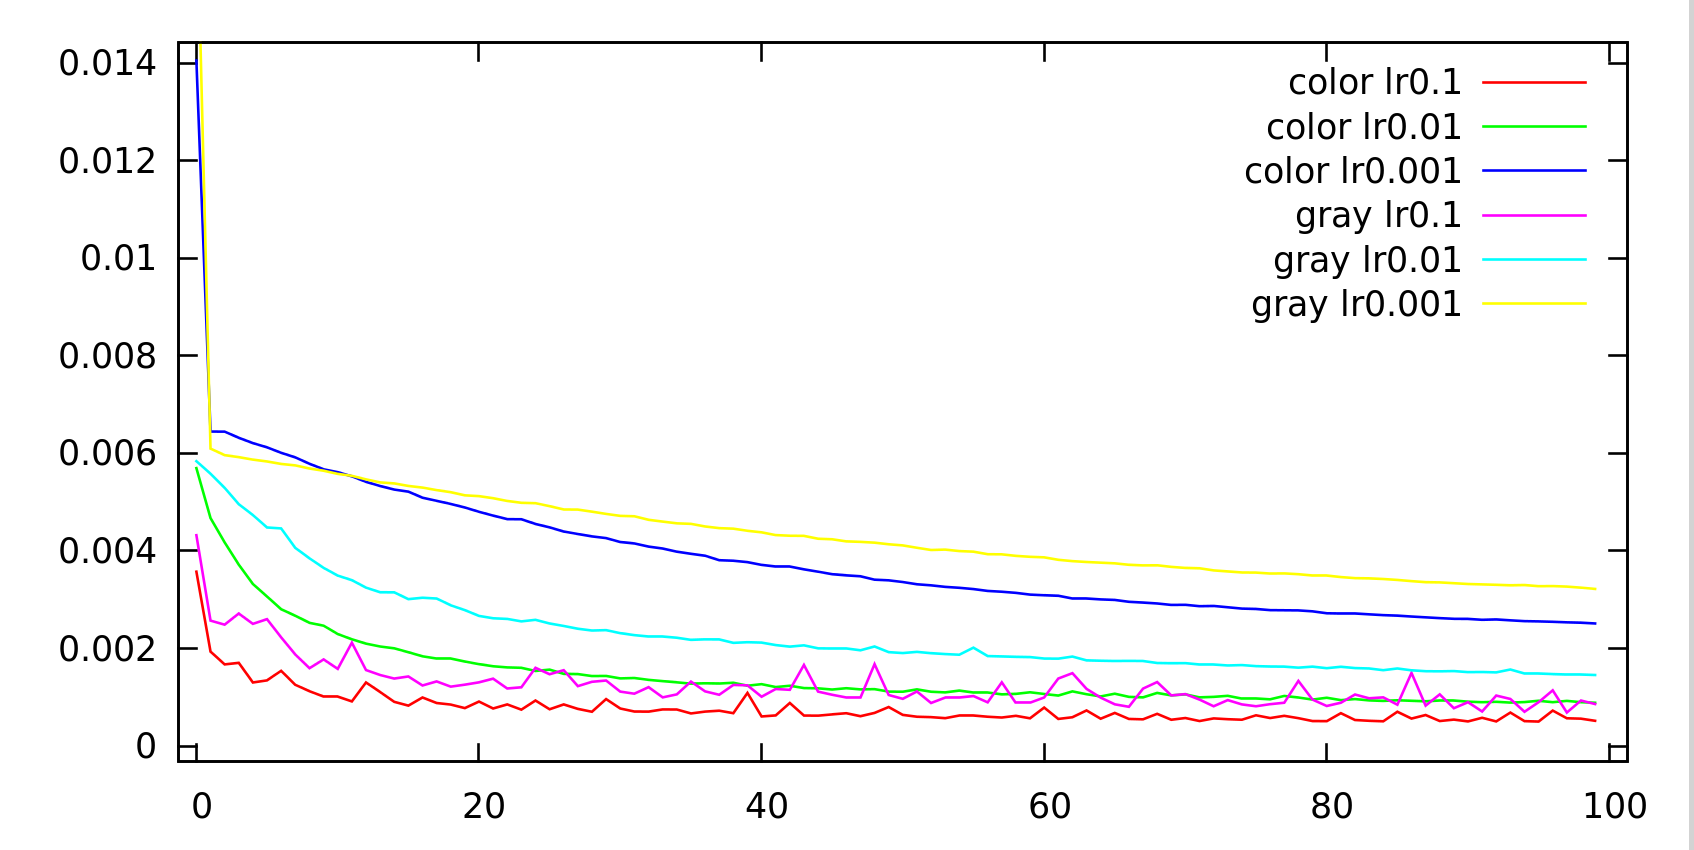
\includegraphics[width=\textwidth]{results/cnn_color_vs_gray.png}
	\caption{Color vs Gray-Value}
	\label{fig:cnn_color_vs_gray}
\end{figure}

\subsubsection{96$\times$128 vs 120$\times$160}

\subsubsection{Glorot Uniform vs Glorot Normal}

\subsubsection{Learningrates}

\subsubsection{Momentum}

\subsubsection{Decay}

\subsubsection{More epochs}

\subsubsection{Larger fully connected layers}

\subsubsection{Larger filters}

Gridsearch, Momentum (bad!?), Decay (bad, too!?), Color vs no color

\subsection{Gabor Networks}

\subsubsection{Absolute Value and Phase}

Errors after 1000 training epochs.

\tiny
\begin{tabular}{|l|l|l|l|l|}
\hline
	\textbf{Setup} & \textbf{Training error} & \textbf{Training error (pixels)} & \textbf{Test error} & \textbf{Test error (pixels)}\\
\hline
	2cl complete 2000 & 5.0980641299870449e-05 & 1.1424116671658617 & 0.00043121594174221544 & 3.322518338339266\\
\hline
	2cl complete 1500 & 6.8641028017271848e-05 & 1.3255980979324613 & 0.00045517455199553872 & 3.4135712283597934\\
\hline
	2cl & 7.3192541588294461e-05 & 1.368842235124391 & 0.00031657626308453598 & 2.846814418778316\\
\hline
	largerconv & 7.5359985959604279e-05 & 1.3889620731200218 & 0.00039507331637073795 & 3.1802322083600894\\
\hline
	noconv & 0.00017174116032 & 2.096800826 & TBD & TBD\\
\hline
	lin. dropout05 & 0.00042446642619407908 & 3.2964132796978634 & 0.00067438261828578971 & 0.00067438261828578971\\
\hline
	lin. dropout & 0.00019879159818321658 & 2.2558955901127926 & 0.00050907034532421695 & 3.610013966773529\\
\hline
	linear & 0.00015014586131201213 & 1.9605443248209184 & 0.00054484549607827022 & 3.7347081143783805\\
\hline
	np & 0.00012644284201810042 & 1.7991488975800116 & 0.0006120212749442589 & 3.958250199087095\\
\hline
	old\_p & 0.0001238262047248818 & 1.7804355761883028 & 0.00054604860983845668 & 3.7388292835945975\\
\hline
	color ld & 0.00011004619286889145 & 1.342757172374781 & 0.00040994517442226796 & 2.591629166708547\\
\hline
\end{tabular}

\normalsize

\begin{figure}[htbp]
	\centering
	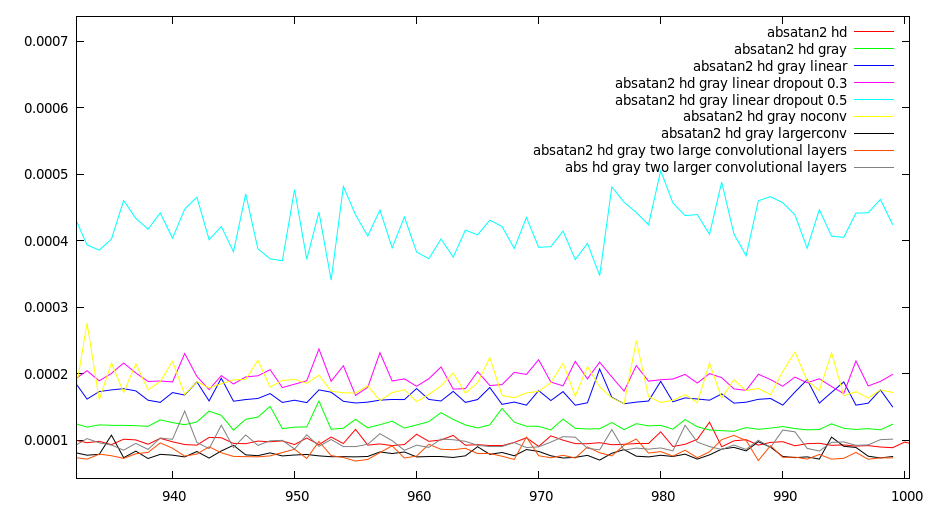
\includegraphics[width=\textwidth]{results/absatan2_and_abs_1.png}
	\caption{Results for all absatan2 and abs networks after 1000 epochs}
	\label{fig:absatan2_results}
\end{figure}

\begin{figure}[htbp]
	\centering
	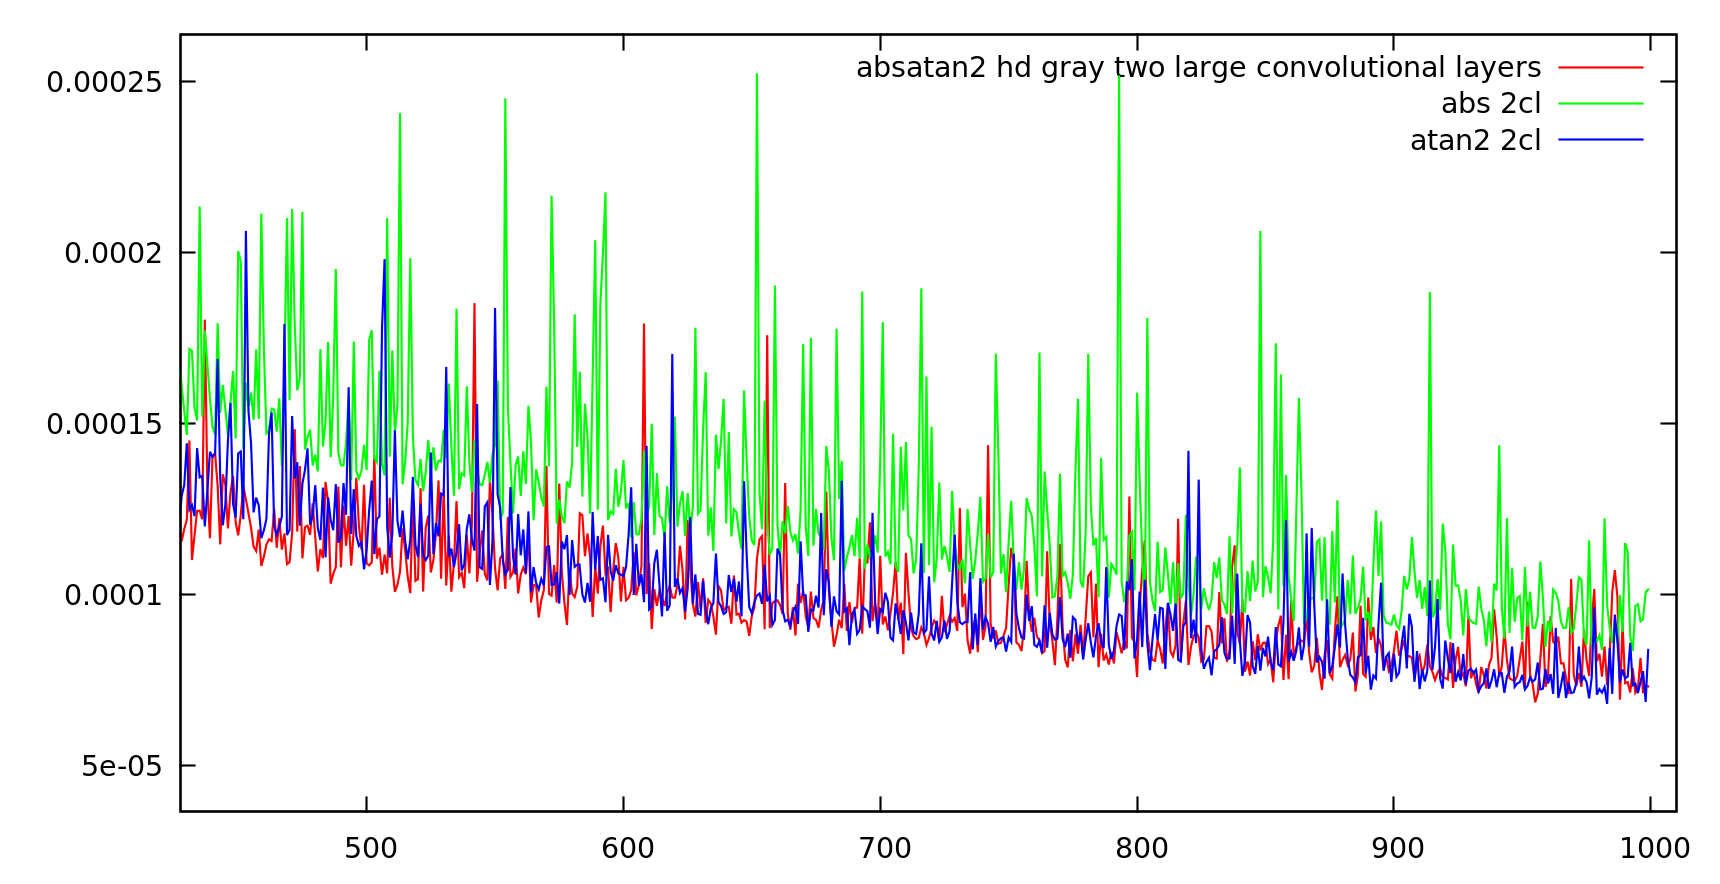
\includegraphics[width=\textwidth]{results/gabor_absatan2_vs_atan2_vs_abs.png}
	\caption{Absatan2 vs atan2 vs abs after 1000 epochs}
	\label{fig:gabor_absatan2_vs_atan2_vs_abs}
\end{figure}

%TODO Gesamtanzahl der Gewichte bei jedem Netzwerk angeben!

\subsubsection{Absolute Value}
\subsubsection{Phase}

\newpage

%%%%%%%%%%%%%%%%%%%%%%%%%%%%%%%%%%%%%%%%%%%%%%%%%%%%%%%%%%%%%%%%%%%%%%%%%%%%%%%%%%%%%%%%%%%%%%%%%%%%%%%%%
%%%%%%%%%%%%%%%%%%%%%%%%%%%%%%%%%%%%%%%%%%%%%%%%%%%%%%%%%%%%%%%%%%%%%%%%%%%%%%%%%%%%%%%%%%%%%%%%%%%%%%%%%
%									CONCLUSION CHAPTER BEGINS HERE										%
%%%%%%%%%%%%%%%%%%%%%%%%%%%%%%%%%%%%%%%%%%%%%%%%%%%%%%%%%%%%%%%%%%%%%%%%%%%%%%%%%%%%%%%%%%%%%%%%%%%%%%%%%
%%%%%%%%%%%%%%%%%%%%%%%%%%%%%%%%%%%%%%%%%%%%%%%%%%%%%%%%%%%%%%%%%%%%%%%%%%%%%%%%%%%%%%%%%%%%%%%%%%%%%%%%%

\section{Conclusion}
\label{sec:conclusion}

\newpage

%%%%%%%%%%%%%%%%%%%%%%%%%%%%%%%%%%%%%%%%%%%%%%%%%%%%%%%%%%%%%%%%%%%%%%%%%%%%%%%%%%%%%%%%%%%%%%%%%%%%%%%%%
%%%%%%%%%%%%%%%%%%%%%%%%%%%%%%%%%%%%%%%%%%%%%%%%%%%%%%%%%%%%%%%%%%%%%%%%%%%%%%%%%%%%%%%%%%%%%%%%%%%%%%%%%
%										APPENDIX BEGINS HERE											%
%%%%%%%%%%%%%%%%%%%%%%%%%%%%%%%%%%%%%%%%%%%%%%%%%%%%%%%%%%%%%%%%%%%%%%%%%%%%%%%%%%%%%%%%%%%%%%%%%%%%%%%%%
%%%%%%%%%%%%%%%%%%%%%%%%%%%%%%%%%%%%%%%%%%%%%%%%%%%%%%%%%%%%%%%%%%%%%%%%%%%%%%%%%%%%%%%%%%%%%%%%%%%%%%%%%

\begin{appendix}
\label{appendix}

\section{Implementation Remarks}
The neural networks discussed in this thesis were implemented with the highly modular and easily extensible neural network library Keras \cite{keras}, which is written in Python and uses TensorFlow or Theano \cite{theano} as backend. Keras supports many different network kinds like fully connected feed-forward networks, \acp{CNN}, \acp{RNN} and combinations of these network types and provides an ample range of pre-defined layers, objective functions, optimization methods, activation functions and initialization methods. The delivered functionality should in general be sufficiently comprehensive to construct any desired network architecture. Network components, which are not part of the library yet, can usually be programmed by the network designer without difficulty. In the scope of this thesis, Keras has been used with Theano as backend. Theano is a powerful mathematical library, which runs on the \ac{GPU} and is thus significantly faster than a program executed on the \ac{CPU} (which is possible in Keras, too). Theano is closely linked with NumPy and works on symbolic mathematical expressions, which allow for automatically computable derivatives. This is an extremely invaluable feature, because it is not necessary to calculate the network's gradients, which are required for Backpropagation, by hand. Quite the contrary, it is sufficient to define a neural network with its error function and all its inputs, outputs, layers and activations functions and Keras will be able to compute the derivatives with respect to the weights only by means of Theano. Another advantage of Keras is that the weights can be conveniently saved to the file system in the \ac{HDF} -- or more specifically the HDF5 format (cf. \cite{hdf5}). This file format has been developed by the HDF Group in order to facilitate the storage of huge amounts of data organized in tables. Since the weight matrices of the layers are tables, \ac{HDF}5 is the ideal format to save them. A nice tool to visualize the weight matrices is hdfview developed by the same group.\\
This chapter is meant to concisely introduce the Keras components, from which the examined networks were constructed. Much more detailed annotations and exemplifications can be found in the respective documentations on the internet (\url{http://deeplearning.net/software/theano/} and \url{http://www.keras.io}).

\subsection{Conventional CNN}

The conventional \acp{CNN} used for the first experiments were composed of three very basic Keras layers, namely the \texttt{Convolution2D}-layer, the \texttt{MaxPooling2D}-layer and the \texttt{Dense}-layer for the fully connected layers. In order to construct a network in Keras, these layers have to be added to a model. The basic Keras model is the \texttt{Sequential} model, which allows to define a network with subsequent layers.\\
The \texttt{Convolution2D}-layer works as described in chapter \myref{subsubsec:convolutionallayer} and \myref{subsubsec:maps}. It takes a certain number of input maps and produces a certain number of output maps, using as many filters as the product of the aforementioned map counts. It is important to mention that the way how Keras named its variables may be confusing. The parameter \texttt{nb\_filters} does not define the number of filters but the number of output maps.\\
The \texttt{MaxPooling2D} layer operates according to chapter \myref{subsubsec:maxpoolinglayer}. The two most important parameters are the \texttt{pool\_size} and the \texttt{strides}. The \texttt{pool\_size} is a tuple which defines the size of the two-dimensional pooling region. Under the assumption that the pooling region is moved over the input map without overlap and without leaving out any neurons, the two values of the \texttt{pool\_size} equal the factors by which the map is downscaled. The \texttt{strides} tuple defines how many rows and columns are skipped after each pooling operation. This way it is possible to let overlap several pooling regions or to completely skip some rows and columns. The \texttt{strides} were always set equal to the \texttt{pool\_size} in order to avoid redundancy and to use all information present in the input map.\\
The \texttt{Dense} layer corresponds to the fully connected layers found in chapter \myref{subsec:feed_forward_neural_networks}. It takes an integer as number of neurons and connects each neuron of the previous layer with each of its own neurons. They are used to combine the responses obtained from the convolutional and max pooling layers logically in order to produce reasonable predictions.

\subsection{Gabor Layer}
	
The functionality of the Gabor layer was explained in chapter \myref{subsubsec:gaborlayer}, the realization of this layer in Keras, however, turns out to be a bit more complicated, because there is no already existing layer, which fulfills the requirements of the Gabor layer.  Fortunately, a layer with the desired behavior can be composed of other Keras layers like the \texttt{Convolution2D}-layer and the \texttt{Merge}-layer. The latter layer is crucial for the realization of the Gabor layer, because it allows to compose complex network architectures by combining several \texttt{Sequential} models into one model.\\
Firstly, it is necessary to implement the convolution of the input image with the real and the imaginary filters. One problem in doing so is that Keras imposes the constraint that all filters within one \texttt{Convolution2D}-layer must have the same size. This may give rise to some difficulties, because the Gabor filters have 5 different sizes (with $M = 5$). Creating one real \texttt{Convolution2D}-layer and one imaginary \texttt{Convolution2D}-layer for each of the 5 filter sizes and applying the operations described below to each pair of real and imaginary layer dissolves this intricateness. The input image is convolved with the 8 real filters and the 8 imaginary filters of each layer pair, yielding 16 output maps per layer pair and 80 output maps in total, which are subsequently inserted into an activation function. The output maps of each pair of  real and imaginary layer are then merged by an \texttt{ExtendedMerge}-layer with one of the two introduced merging operations, resulting in 8 output maps per layer pair and 40 output maps in total. The \texttt{ExtendedMerge}-layer is a modified \texttt{Merge}-layer, which realizes the absolute value merging operation and the phase merging operation, which are both missing in Keras. The merging operations were implemented by means of the \texttt{sqrt} function and the \texttt{arctan2} function of the Theano backend, respectively. Figure \ref{fig:merge_real_imag_one_size} exemplifies the structure of the first stage of Gabor layer by illustrating how one layer pair is merged. The 4 remaining layer pairs with the other filter sizes are treated analogously.
\begin{figure}[htbp]
	\centering
	\newcommand\sfM{0.9}
	\newcommand\gridnode[5]{
		\node (#1) at (#2 + #4 / 2,#3 + #5 / 2) [minimum width=#4cm * \sfM,minimum height=#5cm * \sfM] {};
		\draw[step=0.1] (#2 - 0.001,#3 - 0.001) grid (#2+#4 + 0.001,#3+#5 + 0.001);	
	}
	\begin{tikzpicture}[scale=\sfM,every path/.style={>=latex}]
		% draw input image
		\gridnode{inputimage}{7.7}{3}{1.5}{2}
	
		% draw background boxes
		\draw[fill=lightgray] (0,1.5) rectangle (7.7,0);
		\draw[fill=lightgray] (9,1.5) rectangle (16.7,0);
	
		% draw real filters
		\foreach \x in {0,...,7}
		{
			\gridnode{r\x}{0.9 * \x + 0.5}{0.5}{0.4}{0.4}
			\node at (0.9 * \x + .5, 1) [draw,fill=white,inner sep=0pt,minimum size=0.25cm * \sfM] {$*$};
			\draw[->] (inputimage.south) to (r\x.north);
			\node (ar\x) at (0.9 * \x + 0.7, -0.8) [draw,rectangle,minimum size=0.5cm] {};
			\draw[-] (0.9 * \x + 0.55, -0.9) to (0.9 * \x + 0.75,-0.9) to (0.9 * \x + 0.85, -0.7);
			\draw[->] (r\x.south) to (ar\x.north);
		}
		
		% draw imaginary filters
		\foreach \x in {0,...,7}
		{
			\gridnode{i\x}{0.9 * \x + 9.5}{0.5}{0.4}{0.4}
			\node at (0.9 * \x + 9.9, 1) [draw,fill=white,inner sep=0pt,minimum size=0.25cm * \sfM] {$*$};
			\draw[->] (inputimage.south) to (i\x.north);
			\node (ai\x) at (0.9 * \x + 9.7, -0.8) [draw,rectangle,minimum size=0.5cm] {};
			\draw[-] (0.9 * \x + 9.55, -0.9) to (0.9 * \x + 9.75,-0.9) to (0.9 * \x + 9.85, -0.7);
			\draw[->] (i\x.south) to (ai\x.north);
		}
		
		% draw merge operators
		\foreach \x in {0,...,7}
		{
			\node (m\x) at (\x * 2 + 1.35,-2.5) [draw,rectangle] {\footnotesize merge op};
			\draw[->] (ar\x.south) to (m\x.north);
			\draw[->] (ai\x.south) to (m\x.north);
		}
		
		% draw output maps
		\foreach \x in {0,...,7}
		{
			\gridnode{o\x}{\x * 2 + 0.7}{-4.8}{1.3}{1.6}
			\draw[->] (m\x.south) to (o\x.north);
		}
		
		% draw text nodes
		\node at (6,4) {Input image};
		\node at (4,2.4) {8 real filters};
		\node at (13.5,2.4) {8 imaginary filters};
		\node at (8.5,-5.2) {8 output maps};
	\end{tikzpicture}
	\caption{Merging the real and the imaginary filters of one size}
	\label{fig:merge_real_imag_one_size}
\end{figure}


Merging each of the 5 real layers with its corresponding imaginary layer yields 40 output maps, that are divided into 5 groups, each of which with a different map size. Since the first classical convolutional layer demands a fixed number of equally sized maps as input, it is necessary to merge the 5 merged layers with different sizes into one single layer with only one map size. Before explaining how this is done, it is important to explain the nomenclature of the following figure \ref{fig:complete_gabor_layer}, which shows how the complete Gabor layer is constructed from its individual components. It uses the term \q{One Size Gabor} for those parts of the Gabor layer, which work on filters of one size only (cf. figure \ref{fig:merge_real_imag_one_size}). The leftmost One Size Gabor layer, which convolves the input image with the largest filters, produces the smallest output maps and the second from the left One Size Gabor layer produces the second smallest output maps and so on. Larger filters produce smaller output maps than smaller filters, because the border of the input image, which can not be taken into consideration, increases proportionally to the size of the filter.\\
The solution to the problem of the different map sizes is solved by applying zero-padding to all 32 output maps, which are smaller than the 8 largest output maps. In the figure, this is illustrated by the 5 \q{ZeroPadding2D}-layers, which place the small output maps in their center and add as many zeros around them as are required to equate the size of the smaller maps with the size of the largest maps. The output of these 5 layers are 40 output maps of the same size, which have to be merged into one single layer, before they can be passed as input to the subsequent \texttt{Convolution2D}-layer. This is done by a very simple \texttt{Merge}-layer, which does nothing else than combining all its input maps into one single layer without any modification.
\begin{figure}[h!]
	\centering
	\newcommand\sfG{0.7}
	\newcommand\gridnode[5]{
		\node (#1) at (#2 + #4 / 2,#3 + #5 / 2) [minimum width=#4cm * \sfG,minimum height=#5cm * \sfG] {};
		\draw[step=0.1] (#2 - 0.001,#3 - 0.001) grid (#2+#4 + 0.001,#3+#5 + 0.001);	
	}
	\begin{tikzpicture}[scale=\sfG,every path/.style={>=latex}]
		% draw input image
		\gridnode{inputimage}{9.5}{3}{2.1}{2.8}
		
		% draw one size gabor layers
		\foreach \x in {0,...,4}
		{
			\node (osg\x) at (\x * 4.5 + 1.55,1) [draw,rectangle,minimum height=1cm * \sfG] {\footnotesize One Size Gabor};
			\draw[->] (inputimage.south) to (osg\x.north);
		}
		
		% draw representatives for the 40 outputs
		\gridnode{r0}{1.2}{-1.7}{0.6}{0.8}
		\gridnode{r1}{5.6}{-1.9}{0.9}{1.2}
		\gridnode{r2}{9.9}{-2.1}{1.2}{1.6}
		\gridnode{r3}{14.3}{-2.3}{1.5}{2.0}
		\gridnode{r4}{18.7}{-2.5}{1.8}{2.4}
		
		% draw connections to the representatives and add $x8$
		\foreach \x in {0,...,4}
		{
			\draw[->] (osg\x) to (r\x);
			\node at (\x * 4.7 + 2.3,-1.4) {$\times 8$};
		}
		
		% draw zero padding layers
		\foreach \x in {0,...,4}{
			\node (zp\x) at (\x * 4.5 + 1.55,-3.6) [draw,rectangle,minimum height=1cm * \sfG] {\footnotesize ZeroPadding};
			\draw[->] (r\x) to (zp\x);
		}
		
		% draw zero-padded maps
		\foreach \x in {0,...,4}
		{
			\gridnode{zpm\x}{\x * 4.5 + 0.7}{-7}{1.8}{2.4}
			\draw[->] (zp\x) to (zpm\x);
			\node at (\x * 4.5 + 3,-5.8) {$\times 8$};
		}
		
		% draw merge layer
		\node (mergelayer) at (10.55,-8.1) [draw,rectangle,minimum width=22cm * \sfG,minimum height=0.9cm * \sfG] {\footnotesize Merge layer};
		
		% draw connections from zero padded maps to merge layer
		\foreach \x in {0,...,4}{	\draw[->] (zpm\x.south) to (\x * 4.5 + 1.6,-7.65);	}
		
		\draw[->] (mergelayer.south) -- ++(0,-1);
		\node at (10.55,-9.9) {40 output maps};
		\node at (10.55, 6.3) {Input map};
	\end{tikzpicture}
	\caption{The complete Gabor layer}
	\label{fig:complete_gabor_layer}
\end{figure}


In the case that both merging operations shall be used in the same network, there is not only one \texttt{ExtendedMerge}-layer in the One Size Gabor layer but two. Hence, both \texttt{ExtendedMerge}-layers work on the same convolution results but produce twice as many maps in total, because both merging operations are applied to all output maps of the convolution. The output maps of the \texttt{ExtendedMerge}-layers are then merged into one single layer, which becomes the input of the corresponding \texttt{ZeroPadding2D}-layer. Thus, the "$\times 8$" annotations in figure \ref{fig:complete_gabor_layer} have to replaced by "$\times 16$" and the very last \texttt{Merge}-layer of the Gabor layer produces 80 output maps instead of 40.\\
\end{appendix}

\newpage

\addcontentsline{toc}{section}{List of Figures}
\listoffigures

\newpage

\addcontentsline{toc}{section}{References}
\bibliography{ref}{}
\bibliographystyle{alpha}
%http://www.cs.toronto.edu/$\sim$tijmen/csc321/slides/lecture\_slides\_lec6.pdf\\
%http://cs231n.github.io/neural-networks-3/

\newpage

\thispagestyle{empty}

\begin{center}
\subsection*{Erklärung / Declaration}
\end{center}
\vspace{0.5cm}
Ich erkläre, dass das Thema dieser Arbeit nicht identisch ist mit dem Thema einer von mir bereits für eine andere Prüfung eingereichten Arbeit.\\
Ich erkläre weiterhin, dass ich die Arbeit nicht bereits an einer anderen Hochschule zur Erlangung eines akademischen Grades eingereicht habe.

\vspace{0.8cm}
Ich versichere, dass ich die Arbeit selbstständig verfasst und keine anderen als die angegebenen Quellen benutzt habe. Die Stellen der Arbeit, die anderen Werken dem Wortlaut oder dem Sinn nach entnommen sind, habe ich unter Angabe der Quellen der Entlehnung kenntlich gemacht. Dies gilt sinngemäß auch für gelieferte Zeichnungen, Skizzen, bildliche Darstellungen und dergleichen.

\vspace{2cm}
I declare that the topic of this thesis is not identical to the topic of another thesis authored by me for another examination. Furthermore I declare that I did not submit this thesis to another university for the purpose of obtaining an academic degree.

\vspace{0.8cm}
I assure that I composed this thesis thoroughly on my own without using other sources than the denoted ones. Those fragments of this thesis, which are taken literally or figuratively from other works, are indicated by citing their origin. This also applies to the provided drawings, sketches, illustrations and suchlike.

\vspace{1.5cm}
\rule[0.05cm]{5cm}{0.5pt} \hspace{4.5cm} \rule[0.05cm]{5cm}{0.5pt}\\
Datum / Date \hspace{7.1cm} Unterschrift / Signature

\end{document}